\documentclass[11pt]{article}
\usepackage[margin=1.15in]{geometry}
\usepackage{xcolor}
\usepackage{amsmath,amssymb,amsthm,mathtools,booktabs,longtable,graphicx,enumitem,hyperref,cleveref,microtype,xurl}
\graphicspath{{../figures/}}
\hypersetup{colorlinks=true,linkcolor=blue!50!black,citecolor=blue!50!black,urlcolor=blue!50!black,
 pdftitle={Generative Histories, Arithmetic Recombination, and Higher-Dimensional Route Topology},
 pdfauthor={UNNS Research Collective},
 pdfsubject={Manuscript II of the GEO-HD-1 programme: histories of the SELECT-II integer grammar},
 pdfkeywords={integer dynamics; generative history; valuation threshold; swap class; route complex; integer kernel; block rewrite}}
\theoremstyle{plain}
\newtheorem{theorem}{Theorem}[section]
\newtheorem{lemma}[theorem]{Lemma}
\newtheorem{proposition}[theorem]{Proposition}
\newtheorem{corollary}[theorem]{Corollary}
\theoremstyle{definition}
\newtheorem{definition}[theorem]{Definition}
\newtheorem{example}[theorem]{Example}
\newtheorem{problem}[theorem]{Problem}
\theoremstyle{remark}
\newtheorem{remark}[theorem]{Remark}
\crefname{theorem}{Theorem}{Theorems}\crefname{lemma}{Lemma}{Lemmas}\crefname{proposition}{Proposition}{Propositions}
\crefname{corollary}{Corollary}{Corollaries}\crefname{definition}{Definition}{Definitions}\crefname{example}{Example}{Examples}
\crefname{section}{Section}{Sections}\crefname{figure}{Figure}{Figures}\Crefname{figure}{Figure}{Figures}
\crefname{appendix}{Appendix}{Appendices}\crefname{problem}{Problem}{Problems}\crefname{remark}{Remark}{Remarks}
% ---- notation
\newcommand{\Z}{\mathbb Z}\newcommand{\Q}{\mathbb Q}\newcommand{\N}{\mathbb N}\newcommand{\F}{\mathbb F}
\newcommand{\vp}{v}            % valuation v_p
\newcommand{\Dl}{\Delta}       % Delta_p(N)
\newcommand{\kap}{\kappa}
\newcommand{\lcm}{\operatorname{lcm}}
\newcommand{\den}{\operatorname{den}}
\newcommand{\Hh}{\mathcal H}
\newcommand{\Adm}{\mathcal A}
\newcommand{\Fe}{\mathrm{Feas}}
\newcommand{\rank}{\operatorname{rank}}
\newcommand{\Kmove}{K_{\mathrm{move}}}
\newcommand{\stat}[1]{{\upshape\textsc{#1}}}
% provenance line: \prov{uid}{source id}{status}{treatment}
\newwrite\provw
\immediate\openout\provw=\jobname.prov
\newcommand{\provrow}[6]{\texttt{#1} & \texttt{#2} & #3 & #4 & #5 & #6}
\newcommand{\prov}[4]{\par\smallskip\noindent{\footnotesize\textit{Source record:} \texttt{#2} (\texttt{#1}); status \textsc{#3}; treatment \textsc{#4}.}\par
 \immediate\write\provw{\string\provrow{#1}{#2}{#3}{#4}{\thesection}{\thetheorem}}}
% derived allocation (not part of the 518-row crosswalk): \provx{label}{source}{status}{treatment}
\newcommand{\provx}[4]{\par\smallskip\noindent{\footnotesize\textit{Derived allocation:} \texttt{#2} (\texttt{#1}, outside the 62 allocated rows); status \textsc{#3}; treatment \textsc{#4}.}\par
 \immediate\write\provw{\string\provrow{#1}{#2}{#3}{#4}{\thesection}{\thetheorem}}}
\title{Generative Histories, Arithmetic Recombination,\\ and Higher-Dimensional Route Topology}
\author{UNNS Research Collective\\[2pt]\small Manuscript II of the programme \emph{GEO-HD-1} --- version 0.4}
\date{2 November 2026}
\setlength{\emergencystretch}{2em}
\renewcommand{\topfraction}{0.9}\renewcommand{\bottomfraction}{0.8}\renewcommand{\textfraction}{0.08}\renewcommand{\floatpagefraction}{0.6}\setcounter{topnumber}{3}\setcounter{totalnumber}{4}
\begin{document}
\maketitle
\begin{abstract}
On the positive integers consider the moves $m\mapsto m(N+1)^2/N$, admissible whenever the label $N$ divides $m$. A \emph{history} is a finite sequence of such moves. We show that the history, and not the integer it reaches, is the mathematical object that carries the arithmetic and the topology of this system.

Histories ending at one integer are counted exactly by a recursion over the squares dividing the endpoint, with a binomial lower bound along a family. Whether a word of labels is admissible from a given source is decided by a single divisibility $K(w)\mid m$, where $K(w)$ is a product of prime powers read off the valuation walk. From this we obtain a diamond criterion, a saturation theorem, a classification of swap classes for a family of three labels, a block factorisation of the swap graph along the strongly connected components of a feeding digraph, and the exact classification of three-label contents. Complexes of feasible label subsets inside the permutohedron are studied by Alexander duality: a complementary pair of infeasible subsets gives the homology of a sphere, realised by explicit loops and voids.

Histories with different contents reach one endpoint exactly when the content difference lies in the integer kernel of a valuation matrix. We realise every kernel vector, give the exact admissibility threshold of a block rewrite, separate algebraic, exposure and emptiness obstructions, and prove an exposure dichotomy for an infinite family. Finally, an occurrence-event invariant separates histories of one endpoint although the geometry of that endpoint is contractible. Finite-exact computations are kept separate from theorems throughout.
\end{abstract}
\tableofcontents
\section{Introduction and contributions}\label{sec:intro}
We study the dynamics on the positive integers in which a state $m$ moves to
\[
 T_N(m)=m\,R(N),\qquad R(N)=\frac{(N+1)^2}{N},
\]
whenever the \emph{label} $N\ge1$ divides $m$. In the UNNS programme this is the integer grammar SELECT-II~\cite{FoundI,RefColl}; Manuscript~I~\cite{PaperI} studied the geometry carried by a single state of the programme's arithmetic, and the present manuscript studies what happens \emph{between} states. A finite sequence of such moves is a \emph{history}. The point of view taken here is that the history is a mathematical object in its own right: it has an arithmetic (which words of labels are admissible from which sources), a combinatorics (how many histories end at one integer, how adjacent exchanges connect them) and a topology (cell complexes whose vertices are histories), and none of this is recoverable from the integer at which a history ends.

\paragraph{The four histories of $72$.}
The integer $72$ is reached from four complete histories (\cref{fig:objects}, \cref{fig:four}):
\[
 1\to4\to16\to72,\qquad 1\to4\to18\to72,\qquad 3\to16\to72,\qquad 10\to72 .
\]
The first two have the same source, content $\{1,1,2\}$ and endpoint, and differ by one exchange of adjacent labels; the third and fourth have other contents altogether. The same endpoint hides three contents and three swap classes. The contribution of this manuscript is to show that this phenomenon is governed by exact arithmetic that can be stated and proved, and to chart the topology it produces.

\begin{figure}[tbp]\centering
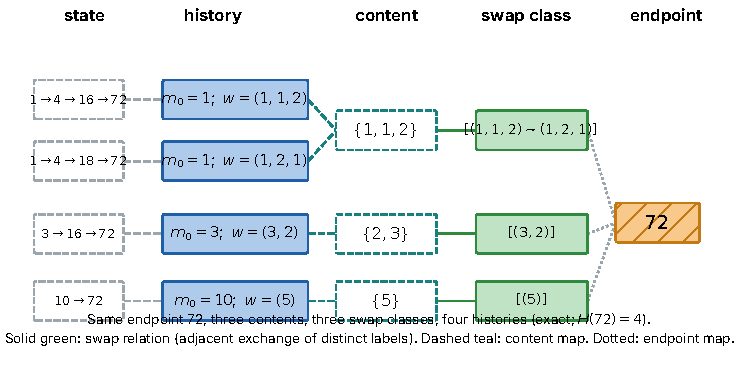
\includegraphics[width=\textwidth]{fig01_objects}
\caption{\textbf{Objects and equivalence relations (exact, endpoint $72$).} The four complete histories ending at $72$ (middle left, with their state sequences in dashed boxes), their three contents, the swap classes they fall into, and the common endpoint. Source $m_0$ and word $w$ are as in \cref{def:history}; the swap relation is \cref{def:swapgraph}.}\label{fig:objects}
\end{figure}

\paragraph{Contributions.}
The results are organised in nine groups, HII-1 to HII-9; each is a part of the programme's allocation for Manuscript~II and is tagged in the text by the identifiers of the source records it restates (\cref{app:crosswalk}).
\begin{enumerate}[leftmargin=2.2em,itemsep=2pt]
\item[\textbf{HII-1}] \emph{Complete ancestry and counting} (\cref{sec:ancestry}). The predecessors of an integer $t$ correspond to the squares $d^2\mid t$; $H(t)=\sum_{d^2\mid t}H(t(d-1)/d^2)$ with $H=1$ on squarefree $t$, and the recursion terminates because $R(N)\ge4$ (\cref{thm:predecessors}). $H(72)=4$, $H(72^r)\ge\binom{2r}{r}$ (\cref{prop:growth}), and the exact values for $r\le 6$ are finite-exact computations (\cref{tab:growth}).
\item[\textbf{HII-2}] \emph{Ordered-word admissibility} (\cref{sec:threshold}). A word $w$ is admissible from $m$ iff $K(w)\mid m$, with $K(w)=\prod_p p^{\max(0,\max_j -\sum_{i\le j}\Delta_p(N_i))}$ and $\Delta_p(N)=2v_p(N+1)-v_p(N)$ (\cref{thm:threshold}); the diamond criterion, the prefix-set form, the gcd reduction and the saturation criterion $P(C)\mid m$ follow.
\item[\textbf{HII-3}] \emph{Swaps} (\cref{sec:swaps}). The swap graph at a source is an induced subgraph of the arrangement graph; classes only merge or appear as the source gains divisors; numerical commutativity of the multipliers never implies admissibility; the contents $(14,3,2)$ and $(2,3,14)$ lie in different classes of one source and endpoint, and the number of classes of $\{2,3,14\}$ is classified for every source (\cref{thm:2314}).
\item[\textbf{HII-4}] \emph{Feeding, factorisation and components} (\cref{sec:feeding}). Non-feeding pairs commute; the class count is a product over the strongly connected blocks of the feeding digraph (\cref{thm:F2}); an acyclic feeding digraph forces at most one class; three distinct labels split exactly at antipodal deadlocks (\cref{thm:T3}); $\{2,3,N\}$ has a split source iff $N\equiv2,3\pmod 6$ (\cref{thm:23N}).
\item[\textbf{HII-5}] \emph{Feasible-subset geometry and topological obstructions} (\cref{sec:feasible}). Alexander duality identifies the homology of the permutohedral route complex with that of a nerve of the infeasible arrangements (\cref{thm:dual}); lower sets are contractible; a complementary pair of infeasible subsets gives the homology of $S^{k-3}$ (\cref{thm:sphere}; the homotopy type is not proved), with a loop for $\{2,3,8,9\}$ at $72$ and a void for $\{2,3,8,9,14\}$ at $1008$.
\item[\textbf{HII-6}] \emph{Higher-dimensional complexes} (\cref{sec:complexes}). Commuting swaps give cubes (\cref{lem:indep}); the maximal cube dimension of $72^r$ and the swap-class counts are finite-exact; cube dimension is not homological degree; irreducible prime-resource obstructions (\cref{prop:irred}).
\item[\textbf{HII-7}] \emph{Different-content endpoint relations} (\cref{sec:endpoints}). Same endpoint iff the content difference lies in the integer kernel of a valuation matrix (\cref{thm:kernel}); every kernel vector is realised (\cref{thm:realise}); the integer kernel of $\{1,2,3\}$ is $\mathbb Z(7,-2,-4)$ and gives the histories $4\to 65536$ of \cref{fig:merger}.
\item[\textbf{HII-8}] \emph{Block rewrites, exposure and resources} (\cref{sec:rewrites}). The exact admissibility threshold of a block rewrite (\cref{thm:block}); saturation; the trichotomy algebraic/exposure/emptiness; the exposure dichotomy of $2^4 3^j\leftrightarrow 1\cdot 8^2 3^j$ for all $j$ (\cref{thm:Fj}), and a counterexample showing that a restricted relation set can omit a Graver move (\cref{prop:graver}).
\item[\textbf{HII-9}] \emph{Occurrence events and state geometry} (\cref{sec:events,sec:geometry}). Occurrence-event invariants (births, losses, churn, and the scoped separator $I=[2\text{ before }4]$ of \cref{thm:R3T3}); the contractibility of the endpoint's move complex shows that no homology of state geometry sees the history components (\cref{prop:A4T7}).
\end{enumerate}

\paragraph{What is new in treatment, and what is not claimed.}
Every theorem of this manuscript restates and re-proves a result of the programme's internal releases (listed in \cref{app:crosswalk}); every finite computation not marked \stat{cited} was re-run with an independent exact engine written for this manuscript (\cref{app:examples}, \texttt{scripts/}), and several statements are sharpened or corrected where the re-derivation required it (\cref{sec:synthesis}). \emph{No claim of novelty or priority is made.} Several of the structures resemble known ones---Mazurkiewicz traces and commutation classes~\cite{Mazurkiewicz1987,CartierFoata1969,DiekertRozenberg1995}, rewriting systems and confluence~\cite{Newman1942,BaaderNipkow1998}, Markov and Graver bases of toric ideals~\cite{Graver1975,Sturmfels1996,DiaconisSturmfels1998}, directed topology of concurrent programs with semaphores~\cite{Pratt1991,FajstrupEtAl2016}---and each such resemblance is pointed out where it occurs and is \emph{only} a resemblance: we prove no equivalence with any of them, and the swap relation here depends on the state through divisibility and is not a trace congruence (\cref{rem:traces}). The programme's same-author caveat applies: all proofs and code originate from one author-collective; no independent human review is claimed. The claim C3 of the programme is not made.

\paragraph{Model boundaries.}
The manuscript uses only two models of the programme: the integer grammar SELECT-II (model M0) and the history, route and rewrite complexes built on it (model M6). The rational dynamics FIELD-I and its occurrence geometry~\cite{FoundII} are \emph{not} used, and SELECT-II is never extended to rational states; the correspondence between the integer move complex of an endpoint and the history space is discussed only as a non-relation in \cref{sec:geometry}. The two dynamics are different maps and nothing here identifies them (the programme's erratum on this point is recorded in \cref{app:crosswalk}).

\paragraph{Status vocabulary.}
Statements are labelled \stat{proved} (a complete argument is given in this manuscript), \stat{proved-scoped} (proved under stated hypotheses, with the scope part of the statement), \stat{finite-exact} (an exhaustive exact computation in a stated range, no claim beyond it), \stat{counterexample}, \stat{open} and \stat{cited} (taken from a released source without re-proof). Finite-exact tables are never extrapolated.

\paragraph{Organisation.} \Cref{sec:grammar} fixes the grammar and the vocabulary. \Cref{sec:ancestry,sec:threshold,sec:swaps,sec:feeding} treat counting, admissibility, swaps and their component structure. \Cref{sec:feasible,sec:complexes} treat the topology of the route complexes; \Cref{sec:endpoints,sec:rewrites} the relations between histories with different contents; \Cref{sec:events,sec:geometry} occurrence events and state geometry; \Cref{sec:synthesis} the conclusions and open problems. The appendices give the source crosswalk, the complete examples, the construction of the complexes, the kernel and rewrite calculations, and the supplementary proofs.

\section{Grammar, notation and history spaces}\label{sec:grammar}
\subsection{The grammar}
\begin{definition}[SELECT-II]\label{def:select}
For an integer \emph{label} $N\ge1$ put $R(N)=(N+1)^2/N$ and $T_N(m)=m\,R(N)$. The label $N$ is \emph{admissible at} the integer $m\ge1$ if $T_N(m)\in\mathbb Z$.
\end{definition}
\begin{lemma}[admissibility is divisibility]\label{lem:adm}
For a positive integer $m$, $T_N(m)\in\mathbb Z$ if and only if $N\mid m$.
\end{lemma}
\begin{proof}
$\gcd(N,(N+1)^2)=1$, so $N\mid m(N+1)^2$ iff $N\mid m$.
\end{proof}
\begin{lemma}[multipliers]\label{lem:R}
$R(N)=N+2+1/N$; $R(1)=4$, $R$ is strictly increasing on integers $N\ge1$, and hence $R(N)\ge4$ with equality only for $N=1$. In particular $N\mapsto R(N)$ is injective.
\end{lemma}
\begin{proof}
$R(N+1)-R(N)=1-\frac1{N(N+1)}>0$.
\end{proof}
For a prime $p$ let $v_p$ be the $p$-adic valuation and put
\[
 \Delta_p(N)=v_p\bigl(R(N)\bigr)=2v_p(N+1)-v_p(N),
\]
so at most one of $v_p(N),v_p(N+1)$ is nonzero and $\Delta_p(N)\ge-v_p(N)$ with equality unless $p\mid N+1$. A prime is \emph{active} for a set of labels if it divides one of them. All valuations of $R(N)$ vanish outside the primes dividing $N(N+1)$.

\begin{definition}[history]\label{def:history}
A \emph{history} is a pair $h=(m_0;w)$ with $m_0\in\mathbb Z_{\ge1}$ the \emph{source} and $w=(N_1,\dots,N_l)$ a word of labels such that $m_j=T_{N_j}(m_{j-1})$ is an integer for $j=1,\dots,l$, i.e.\ $N_j\mid m_{j-1}$. The integers $m_0,\dots,m_l$ are the \emph{states} of $h$, $m_l$ is the \emph{endpoint}, $l$ the length, and the multiset of letters of $w$ is the \emph{content}. The history is \emph{complete} if $m_0$ is squarefree (equivalently, by \cref{thm:predecessors}(b), $m_0$ has no predecessor, so the history cannot be extended backwards).
\end{definition}
By \cref{lem:R} states increase strictly, so a history determines the set of its states, and $m_l=m_0\prod_j R(N_j)$ depends only on the source and the content.

\subsection{Vocabulary: state, history, content, endpoint, swap class, rewrite class}
The words are used in a fixed sense throughout.
\begin{itemize}[leftmargin=1.6em,itemsep=1pt]
\item A \emph{state} is an integer $m$. A \emph{history} is a path $(m_0;w)$. Its \emph{content} is the multiset of its labels and its \emph{endpoint} the last state. Two histories have the same endpoint from the same source iff they have the same multiplier $\prod R(N_j)$ (\cref{sec:endpoints}).
\item Two histories of the same source are \emph{swap-adjacent} if their words differ by exchanging two adjacent \emph{distinct} labels (\cref{def:swapgraph}); the connected components of the resulting graph are \emph{swap classes}. Swap classes lie inside content classes, which lie inside endpoint classes.
\item A \emph{block rewrite} replaces a contiguous block of a word by another word of equal multiplier, possibly with a different content (\cref{def:rewrite}); the components of swaps and block rewrites together are \emph{rewrite classes}.
\end{itemize}
\Cref{fig:objects} displays the nesting for the endpoint $72$. A function of the endpoint alone sees none of the finer relations; the manuscript's results are statements about the finer relations.

\subsection{Valuation walks}
For an integer $m$ write $u(m)=(v_p(m))_p$. A step with label $N$ requires $u_p\ge v_p(N)$ for all $p$ and changes $u$ by $\Delta(N)=(\Delta_p(N))_p$. A history is therefore a lattice walk in the nonnegative orthant with step set $\{\Delta(N)\}$: $p$ is a resource of capacity $u_p$, a label divisible by $p$ consumes it, and a label $N$ with $p\mid N+1$ produces it. The total displacement of a walk is determined by the content, so it is the \emph{route} of the walk---not its endpoint---that distinguishes histories. This is the picture behind \cref{thm:threshold} below; it is inherited arithmetic (record \texttt{D-W}).
\prov{CW-0337}{D-W}{PROVED}{FULL}

\begin{remark}[model boundaries]\label{rem:bounds}
Only integer states and the grammar of \cref{def:select} are used. Rational states, the collective map of the programme's FIELD-I, the occurrence geometry of rational states and the move complexes of rational states are not used; where an integer move complex enters (\cref{sec:geometry}) it is the complex of an integer endpoint, which is not a rational extension.
\end{remark}

\section{Complete ancestry and exact counting}\label{sec:ancestry}
\subsection{Predecessors}
\begin{theorem}[predecessors and the count recursion]\label{thm:predecessors}
Let $t\ge1$ be an integer.
\begin{enumerate}[label=(\alph*),itemsep=1pt]
\item $m\xrightarrow{N}t$ (that is, $T_N(m)=t$ with $N\mid m$) if and only if $d:=N+1$ satisfies $d^2\mid t$ and $m=t(d-1)/d^2$. The correspondence $d\leftrightarrow(N,m)$ is a bijection.
\item Hence $t$ has exactly $\#\{d\ge2:\ d^2\mid t\}$ incoming edges, one for each square divisor $d^2\ge4$, and $t$ has none iff $t$ is squarefree.
\item Let $H(t)$ be the number of complete histories ending at $t$. Then $H(t)=1$ for squarefree $t$ and, for every other $t$,
\[
 H(t)=\sum_{d\ge2,\ d^2\mid t}H\!\left(\frac{t(d-1)}{d^2}\right).
\]
\item Every history ending at $t$ from a source $m_0$ has length at most $\log_4(t/m_0)$; in particular $H(t)$ is finite.
\end{enumerate}
\end{theorem}
\begin{proof}
(a) If $m=Nk$ and $T_N(m)=t$ then $t=k(N+1)^2$, so $(N+1)^2\mid t$ and $m=Nt/(N+1)^2$. Conversely, if $d^2\mid t$ and $N=d-1$, put $m=Nt/d^2=N\cdot(t/d^2)$; then $N\mid m$ and $T_N(m)=m\,d^2/N=t$. The two maps are mutually inverse, and $N$ is determined by $d=N+1$.
(b) is the count of the $d$ of (a); $t$ has a square divisor $d^2\ge4$ iff $t$ is not squarefree.
(c) A complete history of a non-squarefree $t$ has positive length, because its source is squarefree. Removing its last edge, which is an incoming edge of $t$ of the form in (a), leaves a complete history ending at the predecessor $m$. The map (history) $\mapsto$ (last edge, remaining history) is a bijection onto pairs consisting of an incoming edge and a complete history of its tail. For squarefree $t$ only the empty history is complete, since $t$ has no incoming edge.
(d) By \cref{lem:R}, $t=m_0\prod R(N_j)\ge4^l m_0$.
\end{proof}
\prov{CW-0336}{D-T0}{PROVED}{FULL}

\begin{remark}
The recursion is the definition of $H$ as a path count in the \emph{predecessor graph} of $t$: the directed graph on all ancestors of $t$ whose edges are the incoming edges of (a). It is acyclic because states strictly increase along edges, so the recursion terminates, and \cref{fig:predecessor} shows it for $t=72$.
\end{remark}

\begin{example}[the four histories of $72$]\label{ex:72}
Since $72=2^33^2$, the squares dividing $72$ are $d^2=4,9,36$ ($d=2,3,6$; $16\nmid72$ and $144>72$), with predecessors $72\cdot1/4=18$ (label $N=1$: $18\cdot4=72$), $72\cdot2/9=16$ (label $2$: $16\cdot\frac92=72$) and $72\cdot5/36=10$ (label $5$: $10\cdot\frac{36}5=72$). Next, $18=2\cdot3^2$ has the single square $9$ with predecessor $18\cdot2/9=4$ (label $2$: $4\cdot\frac92=18$); $16$ has squares $4$ and $16$ ($d=2,4$), with predecessors $16/4=4$ (label $1$) and $16\cdot3/16=3$ (label $3$: $3\cdot\frac{16}{3}=16$); $4$ has the square $4$ with predecessor $1$ (label $1$); and $10,3,1$ are squarefree. Hence
\[
 H(18)=H(4)=H(1)=1,\quad H(16)=H(4)+H(3)=2,\quad H(10)=1,\quad H(72)=1+2+1=4 .
\]
Reading the four paths from the sources $1,1,3,10$ gives
\[
 1\xrightarrow{1}4\xrightarrow{1}16\xrightarrow{2}72,\qquad
 1\xrightarrow{1}4\xrightarrow{2}18\xrightarrow{1}72,\qquad
 3\xrightarrow{3}16\xrightarrow{2}72,\qquad
 10\xrightarrow{5}72 ,
\]
with words $(1,1,2),(1,2,1),(3,2),(5)$ and contents $\{1,1,2\},\{1,1,2\},\{2,3\},\{5\}$. The first two differ by exchanging the adjacent distinct labels $1,2$ at the states $4\to16$, $4\to18$; the states $16$ and $18$ are the two intermediate states of the diamond $4\to 16,18\to72$ (\cref{fig:four}). (All sources are squarefree, so all four histories are complete.)
\end{example}

\begin{figure}[tbp]\centering
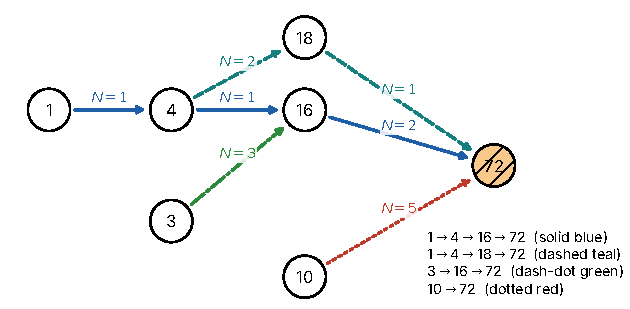
\includegraphics[width=0.92\textwidth]{fig02_four_histories_72}
\caption{\textbf{The four complete histories ending at $72$ (exact).} States are nodes, labels $N$ are edge labels. Source $1$: $1\to4\to16\to72$ (solid blue) and $1\to4\to18\to72$ (dashed teal); source $3$: $3\to16\to72$ (dash-dot green); source $10$: $10\to72$ (dotted red). Theorem illustrated: \cref{thm:predecessors}; \cref{ex:72}.}\label{fig:four}
\end{figure}
\begin{figure}[tbp]\centering
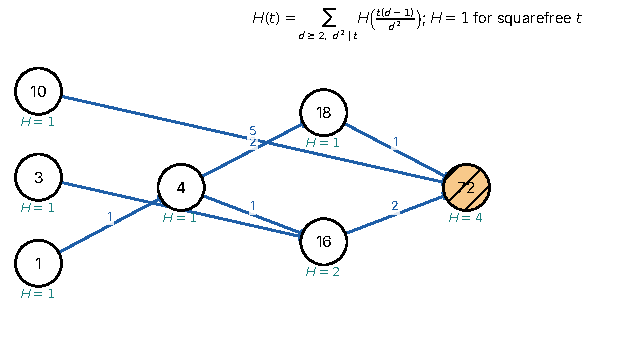
\includegraphics[width=\textwidth]{fig03_predecessor_graph}
\caption{\textbf{Predecessor graph of $72$ and the count recursion (exact).} Nodes are the ancestors of $72$; an edge $s\to t$ carries its label $N$; the number under a node is $H$ of that node, computed by the recursion of \cref{thm:predecessors}(c). $H(72)=4$.}\label{fig:predecessor}
\end{figure}

\subsection{Growth}
\begin{proposition}[lower bound for $72^r$]\label{prop:growth}
For every $r\ge1$, $H(72^r)\ge\binom{2r}{r}$.
\end{proposition}
\begin{proof}
Start from source $1$. Apply the label $1$ exactly $r$ times, reaching $4^r=2^{2r}$ (every state is divisible by the label $1$). We show that every arrangement of $r$ labels $1$ and $r$ labels $2$ is admissible from $4^r$. At a point where $a$ labels $1$ and $b$ labels $2$ have been applied so far, the $2$-adic valuation of the state is $2r+2a-b$, since a label $1$ adds $2$ and a label $2$ changes $v_2$ by $-1$ (the valuation of $R(2)=9/2$ is $-1$ at $2$). Before the $(b+1)$-st label $2$ we have $b\le r-1$, so $v_2\ge 2r-b\ge r+1\ge1$ and $2$ divides the state. The endpoint of any such arrangement is $4^r\cdot4^r\cdot(9/2)^r=72^r$ (the multiplier is $R(1)^rR(1)^rR(2)^r=4^{2r}(9/2)^r=(16\cdot9/2)^r=72^r$). Distinct arrangements are distinct words from one source, hence distinct histories; there are $\binom{2r}{r}$ of them, and the whole history $(1^r)\cdot(\text{arrangement})$ is from source $1$, which is squarefree, so these are complete.
\end{proof}
\prov{CW-0339}{D-T2}{PROVED}{FULL}

\begin{table}[tbp]\centering\small
\begin{tabular}{@{}lrrrrrr@{}}\toprule
$r$ & 1 & 2 & 3 & 4 & 5 & 6\\\midrule
$H(72^r)$ & 4 & 100 & 3\,601 & 194\,864 & 14\,177\,856 & 1\,258\,011\,667\\
$\binom{2r}{r}$ & 2 & 6 & 20 & 70 & 252 & 924\\\bottomrule
\end{tabular}
\caption{\textbf{Counts of complete histories ending at $72^r$ (finite-exact).} Values of $H$ from the recursion \cref{thm:predecessors}(c), computed exactly in this work and agreeing with the programme's records; the bound is \cref{prop:growth}. These are finite computations for $r\le6$: no growth law in $r$ is claimed (it is open, \cref{prob:growth}).}\label{tab:growth}
\end{table}
\begin{figure}[tbp]\centering
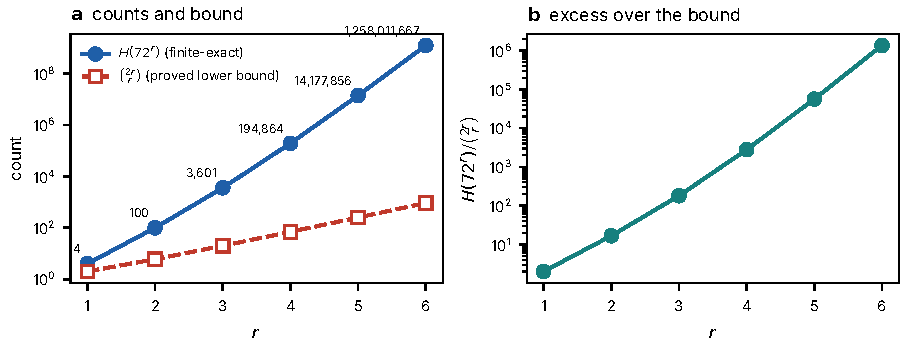
\includegraphics[width=0.95\textwidth]{fig04_growth}
\caption{\textbf{Growth of $H(72^r)$ and its lower bound (finite-exact values, proved bound).} (a) Counts for $r=1,\dots,6$ (circles, \cref{tab:growth}) against $\binom{2r}{r}$ (squares, \cref{prop:growth}). (b) The ratio; the bound is far from sharp.}\label{fig:growth}
\end{figure}
\noindent The figure above is \cref{fig:growth}; its caption states the exactness of what is drawn.
\begin{remark}
The values of \cref{tab:growth} for $r\le4$ were additionally confirmed by enumerating the histories explicitly; the values for $r=5,6$ rest on the recursion, which counts paths in an acyclic graph and whose correctness is \cref{thm:predecessors}.
\end{remark}
\begin{problem}[open: growth]\label{prob:growth}
Determine the asymptotics of $H(72^r)$ (and of the maximum cube dimension, \cref{sec:complexes}). Only the lower bound of \cref{prop:growth} and the finite values of \cref{tab:growth} are known here.
\end{problem}
\prov{CW-0514}{D-Q2}{OPEN}{OPEN}

\section{Ordered-word admissibility and valuation thresholds}\label{sec:threshold}
Fix a word $w=(N_1,\dots,N_l)$ of labels and put $S_j(p)=\sum_{i\le j}\Delta_p(N_i)$, so that $m\prod_{i\le j}R(N_i)$ has $p$-adic valuation $v_p(m)+S_j(p)$.
\begin{definition}[threshold]\label{def:K}
$b_p(w)=\max\bigl(0,\max_{1\le j\le l}(-S_j(p))\bigr)$ and $K(w)=\prod_p p^{\,b_p(w)}$.
\end{definition}
Only the finitely many primes dividing some $N_i(N_i+1)$ contribute.
\begin{theorem}[valuation-threshold theorem]\label{thm:threshold}
$w$ is admissible from $m$ if and only if $K(w)\mid m$. Hence $K(w)$ is the smallest source from which $w$ is admissible, and the admissible sources are exactly the multiples of $K(w)$.
\end{theorem}
\begin{proof}
Put $x_j=m\prod_{i\le j}R(N_i)\in\mathbb Q_{>0}$ (so $x_0=m$). We claim $w$ is admissible from $m$ iff $x_j\in\mathbb Z$ for $j=0,\dots,l$. If $w$ is admissible the $x_j$ are the states. Conversely suppose all $x_j$ are integers; then $x_j=x_{j-1}(N_j+1)^2/N_j$ with $x_{j-1}\in\mathbb Z$, so $x_j\in\mathbb Z$ gives $N_j\mid x_{j-1}$ by \cref{lem:adm}, i.e.\ the step is admissible. Next, a positive rational is an integer iff all its $p$-adic valuations are nonnegative, and $v_p(x_j)=v_p(m)+S_j(p)$. Therefore $w$ is admissible iff $v_p(m)+S_j(p)\ge0$ for all $p$ and $j$, i.e.\ iff $v_p(m)\ge\max_j(-S_j(p))$ for all $p$; since $v_p(m)\ge0$ this is $v_p(m)\ge b_p(w)$ for all $p$, i.e.\ $K(w)\mid m$.
\end{proof}
\prov{CW-0344}{D-T7}{PROVED}{FULL}\prov{CW-0365}{D6-T1}{PROVED}{FULL}
\medskip
For a finite multiset $S$ of labels put $R(S)=\prod_{x\in S}R(x)$ and
\[
 \kappa(S)=\prod_p p^{\max(0,-\sum_{x\in S}\Delta_p(x))}=\den R(S),
\]
the denominator of $R(S)$ in lowest terms (the primes with $v_p(R(S))<0$, to the power $-v_p$). A multiset $S$ is \emph{feasible at $m$} if $\kappa(S)\mid m$, i.e.\ if $mR(S)\in\mathbb Z$.
\begin{corollary}[prefix-set form]\label{cor:P}
$K(w)=\lcm_{1\le j\le l}\ \kappa\bigl(\{N_1,\dots,N_j\}\bigr)$. Consequently $w$ is admissible from $m$ iff every prefix multiset of $w$ is feasible at $m$; and $K(w)$ depends on $w$ only through its prefix multisets.
\end{corollary}
\begin{proof}
$S_j(p)=\sum_{x\in\{N_1..N_j\}}\Delta_p(x)$ depends only on the prefix multiset, so $b_p(w)=\max_j\max(0,-S_j(p))$ is the largest exponent of $p$ among the $\kappa(\text{prefix}_j)$, and the maximum of exponents is the exponent of the lcm.
\end{proof}
\prov{CW-0366}{(P) Prefix-set form}{PROVED}{FULL}
For a single label $\kappa(\{N\})=N$, because $\Delta_p(N)=-v_p(N)$ when $p\mid N$ and $\Delta_p(N)\ge0$ otherwise. For a multiset $C$ let $P(C)=\prod_{x\in C}x$ (with multiplicity).
\begin{corollary}[gcd reduction]\label{cor:G}
For every arrangement $w$ of $C$, $K(w)\mid P(C)$. Hence $w$ is admissible from $m$ iff it is admissible from $\gcd(m,P(C))$.
\end{corollary}
\begin{proof}
Since $\Delta_p(N)\ge-v_p(N)$ we have $-S_j(p)\le\sum_iv_p(N_i)=v_p(P(C))$, so $b_p(w)\le v_p(P(C))$. If $K(w)\mid P(C)$ then $K(w)\mid m\iff K(w)\mid\gcd(m,P(C))$.
\end{proof}
\prov{CW-0367}{(G) Dependence on the source}{PROVED}{FULL}
\begin{proposition}[diamond criterion]\label{prop:diamond}
For labels $A\ne B$: (a) $K\bigl((A,B)\bigr)=AB/\gcd(B,(A+1)^2)$, so $(A,B)$ is admissible from $m$ iff $\frac{AB}{\gcd(B,(A+1)^2)}\mid m$; (b) both $(A,B)$ and $(B,A)$ are admissible from $m$ iff $AB\mid m$; (c) if a history passes through the state $x$ immediately before two adjacent distinct labels $A,B$, then exchanging them gives an admissible history iff $AB\mid x$.
\end{proposition}
\begin{proof}
(a) By \cref{lem:adm}, $A\mid m$, say $m=Ak$, and then $B\mid T_A(m)=k(A+1)^2$. Put $g=\gcd(B,(A+1)^2)$, $B=gB'$, $(A+1)^2=gE$ with $\gcd(B',E)=1$. Then $B\mid kgE$ iff $B'\mid kE$ iff $B'\mid k$. Hence $m=Ak$ with $B'\mid k$, i.e.\ $AB'\mid m$, and $AB'=AB/g$. (b) With $g_1=\gcd(B,(A+1)^2)$ and $g_2=\gcd(A,(B+1)^2)$, both orders are admissible iff $\lcm(AB/g_1,AB/g_2)=AB/\gcd(g_1,g_2)$ divides $m$ (because $g_1,g_2$ divide $AB$, $\lcm(X/g_1,X/g_2)=X/\gcd(g_1,g_2)$). Here $g_1\mid(A+1)^2$ and $g_2\mid A$, so $\gcd(g_1,g_2)\mid\gcd((A+1)^2,A)=1$. (c) The history already admits $(A,B)$ from $x$, so the exchange is admissible iff $(B,A)$ is admissible from $x$, iff (by (b)) $x$ is a multiple of both $K((A,B))$ and $K((B,A))$, i.e.\ of $AB$; and the remainder of the word starts from the same state $xR(A)R(B)$ in both orders.
\end{proof}
\prov{CW-0338}{D-T1}{PROVED}{FULL}
\begin{proposition}[all arrangements; saturation]\label{prop:sat}
For a finite multiset $C$ of labels and a source $m$: every arrangement of $C$ is admissible from $m$ if and only if $P(C)\mid m$. In particular, if $P(C)\mid m$ then every arrangement is admissible and the swap graph of $C$ at $m$ is connected (\cref{def:swapgraph}).
\end{proposition}
\begin{proof}
($\Leftarrow$) By \cref{cor:G}, $K(w)\mid P(C)\mid m$ for every arrangement $w$. ($\Rightarrow$) Fix a prime $p$ and an arrangement that lists first all labels divisible by $p$. These have $\Delta_p(N)=-v_p(N)$ (since $p\nmid N+1$), so after the last of them $S_j(p)=-\sum_iv_p(N_i)=-v_p(P(C))$, and admissibility forces $v_p(m)\ge v_p(P(C))$. For connectivity: the arrangement graph of a multiset under exchanges of adjacent distinct letters is connected, and with all arrangements admissible it is the swap graph.
\end{proof}
\begin{remark}[what is \emph{not} claimed]\label{rem:converse}
\Cref{prop:sat} does \emph{not} say that a connected swap graph forces $P(C)\mid m$: the content $\{2,3,14\}$ has $P=84$ and a connected swap graph at the source $28$ (\cref{thm:2314}). Saturation is a sufficient resource condition for connectivity, not a necessary one; the true thresholds are the path thresholds of \cref{thm:paths}.
\end{remark}
\prov{CW-0368}{D6-T2}{PROVED}{FULL}

\begin{example}[the thresholds of $\{2,3,14\}$]\label{ex:K}
Let $C=\{2,3,14\}$. For $w=(14,3,2)$ the prefix multisets are $\{14\},\{14,3\},\{14,3,2\}$ with $R=\frac{225}{14},\ \frac{225}{14}\cdot\frac{16}{3}=\frac{600}{7},\ \frac{600}{7}\cdot\frac92=\frac{2700}{7}$, whose denominators are $14,7,7$; so $K(14,3,2)=\lcm(14,7,7)=14$. For $w=(2,3,14)$ the prefix products are $\frac92,\ 24,\ \frac{2700}7$ with denominators $2,1,7$ and $K=14$. For $(14,2,3)$ the second product is $\frac{225}{14}\cdot\frac92=\frac{2025}{28}$, so $K=\lcm(14,28,7)=28$; likewise $K(2,14,3)=28$, and $K(3,14,2)=K(3,2,14)=21$ (denominators $3,7,7$ and $3,1,7$). The six thresholds are $14,28,21,21,28,14$ (\cref{fig:valuation,fig:content}). From $m=14$ the two arrangements with threshold $14$ are admissible and both end at $14\cdot\frac{2700}7=5400$.
\end{example}
\begin{figure}[tbp]\centering
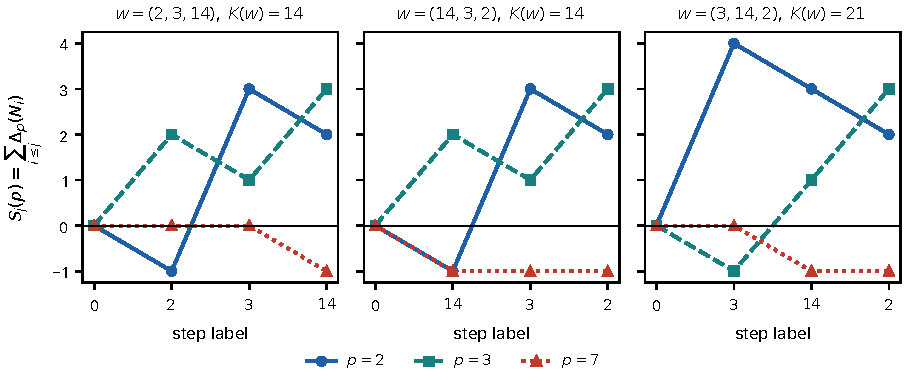
\includegraphics[width=\textwidth]{fig05_valuation_trajectories}
\caption{\textbf{Valuation trajectories of three words of the content $\{2,3,14\}$ (exact).} The curves are $S_j(p)$ for $p=2$ (solid, circles), $3$ (dashed, squares) and $7$ (dotted, triangles); $K(w)=\prod_pp^{\max(0,-\min_jS_j(p))}$ is printed above each panel: $14=2\cdot7$ for $(2,3,14)$ and $(14,3,2)$ (minima $-1$ at $p=2$ and $-1$ at $p=7$) and $21=3\cdot7$ for $(3,14,2)$. Theorem illustrated: \cref{thm:threshold}.}\label{fig:valuation}
\end{figure}
\begin{figure}[tbp]\centering
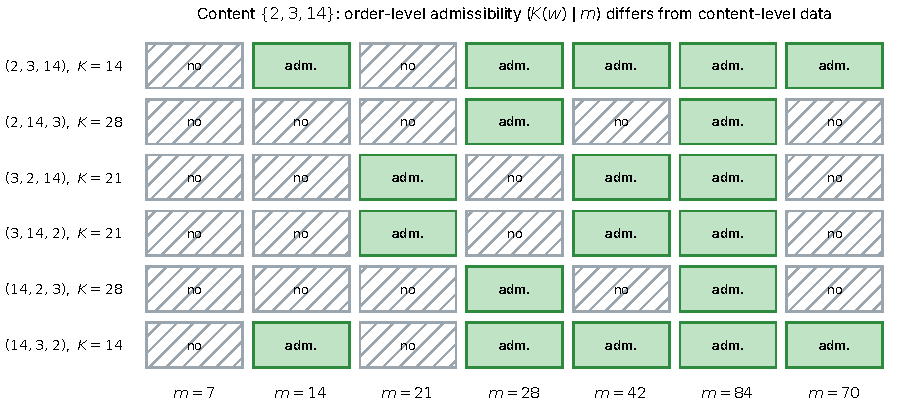
\includegraphics[width=\textwidth]{fig06_content_vs_order}
\caption{\textbf{Content-level versus order-level admissibility for $\{2,3,14\}$ (exact).} Rows: the six arrangements with their thresholds $K$; columns: sources. A cell is filled and marked ``adm.'' iff $K\mid m$. The same content is wholly inadmissible at $m=7$, partly admissible at $m=14$ and $m=21$, and fully admissible among the sources shown only at $m=84=P(C)$ (\cref{prop:sat}); it is connected for $m=28$ (\cref{thm:2314}) although $84\nmid28$.}\label{fig:content}
\end{figure}

\section{Swaps}\label{sec:swaps}
\subsection{The swap graph}
\begin{definition}[arrangement graph, swap graph, swap class]\label{def:swapgraph}
Let $C$ be a finite multiset of labels. The \emph{arrangement graph} $\mathcal G(C)$ has as vertices the distinct arrangements (orderings) of $C$, two being joined if they differ by exchanging two adjacent \emph{distinct} letters. For a source $m$ let $\mathcal A(m)=\{w:K(w)\mid m\}$ be the set of arrangements admissible from $m$. The \emph{swap graph} $\mathrm{Sw}(C,m)$ is the subgraph of $\mathcal G(C)$ induced on $\mathcal A(m)$; its edges are the \emph{legal swaps}, and its components are the \emph{swap classes} of $C$ at $m$. Write $\nu(C,m)$ for their number.
\end{definition}
A vertex of $\mathrm{Sw}(C,m)$ is the history $(m;w)$, and a legal swap is an exchange of adjacent distinct labels of a history that produces an admissible history; the endpoint is unchanged because $m\prod R(N_i)$ does not depend on the order.
\begin{proposition}[the swap graph is an induced subgraph]\label{prop:induced}
The graph on the histories with source $m$ and content $C$, joined by legal swaps, equals $\mathrm{Sw}(C,m)$. In particular two admissible arrangements adjacent in $\mathcal G(C)$ are always joined by a legal swap.
\end{proposition}
\begin{proof}
An edge between two admissible words that differ by an adjacent exchange is, by definition, a legal swap; conversely a legal swap joins two admissible words differing by an adjacent exchange.
\end{proof}
\prov{CW-0345}{D-T7'}{PROVED}{FULL}
\begin{proposition}[numerical commutativity is not admissibility]\label{prop:numcomm}
For all labels $A,B$ the multipliers commute, $R(A)R(B)=R(B)R(A)$, so both orders of $A,B$ have the same endpoint from every source at which both are admissible. Nevertheless the exchange is legal at the state $x$ iff $AB\mid x$ (\cref{prop:diamond}), which is a condition on $x$, not on the multipliers. For instance $(2,3)$ is admissible from $2$ ($2\to9\to48$) while $(3,2)$ is not ($3\nmid2$).
\end{proposition}
\begin{remark}[resemblance to traces and to concurrency]\label{rem:traces}
Adjacent exchanges of commuting letters recall the commutation classes of a trace monoid~\cite{CartierFoata1969,Mazurkiewicz1987,DiekertRozenberg1995}, and the picture of $p$ as a resource of capacity $u_p$ recalls processes with counting semaphores and the directed topology of their state spaces~\cite{Pratt1991,FajstrupEtAl2016}. The resemblance is only that. In a trace monoid independence is a fixed relation on letters; here $A,B$ are interchangeable at $x$ iff $AB\mid x$, which depends on the state, and the classes are not the classes of a congruence on a free monoid. No equivalence with either theory is proved or claimed.
\end{remark}

\subsection{Thresholds of connection; monotonicity}
\begin{theorem}[connection thresholds and the divisibility filtration]\label{thm:paths}
Let $C$ be a multiset and $w,w'$ arrangements of $C$.
\begin{enumerate}[label=(\alph*),itemsep=1pt]
\item $w$ and $w'$ lie in one swap class at the source $m$ iff there is a path $\gamma$ from $w$ to $w'$ in $\mathcal G(C)$ whose threshold $M_\gamma=\lcm_{v\in\gamma}K(v)$ divides $m$. The minimal such $M_\gamma$ form an antichain under divisibility (the \emph{connection thresholds} of the pair).
\item The swap graph depends only on $\mathcal A(m)$. If $m'=\lcm\{K(w):w\in\mathcal A(m)\}$ then $m'\mid m$ and $\mathcal A(m')=\mathcal A(m)$. Hence every swap-graph shape occurring for $C$ occurs at a source in the finite lcm-closure of $\{K(w)\}$, and the classification of $C$ is a finite computation.
\item (\emph{monotonicity}) If $m\mid m^*$ then $\mathcal A(m)\subseteq\mathcal A(m^*)$; the classes at $m^*$ are unions of classes at $m$, together with possibly new classes made of newly admissible arrangements. A class never splits, but $\nu(C,m)$ is not monotone in $m$.
\end{enumerate}
\end{theorem}
\begin{proof}
(a) A path has all its vertices admissible iff every $K(v)$, $v\in\gamma$, divides $m$, iff their lcm does; and a minimal set of thresholds is an antichain by definition. (b) $m'$ divides $m$ since each $K(w)$ with $w\in\mathcal A(m)$ does; $\mathcal A(m')\supseteq\mathcal A(m)$ since those $K(w)$ divide $m'$, and $\mathcal A(m')\subseteq\mathcal A(m)$ because $m'\mid m$. (c) $K(w)\mid m\mid m^*$. For non-monotonicity see the examples below.
\end{proof}
\prov{CW-0346}{D-T8}{PROVED}{FULL}
\begin{example}[class counts are not monotone]\label{ex:nonmono}
For $C=\{2,3,14\}$: $\nu=2$ at $m=14$ and $\nu=1$ at $m=28$ (\cref{thm:2314}). For $C=\{2,3,8\}$ the thresholds are $K(2,3,8)=2$, $K(3,2,8)=K(3,8,2)=3$, $K(8,3,2)=8$, $K(2,8,3)=K(8,2,3)=16$ and one finds $\nu=1,2,1$ at the sources $2,8,16$, which are totally ordered by divisibility: a class count can rise and fall along a divisibility chain.
\end{example}

\subsection{Same content, different swap classes: the source-\texorpdfstring{$14$}{14} example}
\begin{example}[source $14$]\label{ex:src14}
From the source $14$ the content $\{2,3,14\}$ has exactly two admissible arrangements (\cref{ex:K}):
\[
 14\xrightarrow{14}225\xrightarrow{3}1200\xrightarrow{2}5400,\qquad
 14\xrightarrow{2}63\xrightarrow{3}336\xrightarrow{14}5400 .
\]
They have the same source, the same content and the same endpoint $5400$, and neither has a legal swap: exchanging $(14,3)$ at the state $14$ needs $42\mid14$; $(3,2)$ at $225$ needs $6\mid225$; $(2,3)$ at $14$ needs $6\mid14$; and $(3,14)$ at $63$ needs $42\mid63$ --- all four fail by \cref{prop:diamond}(c). The mechanism is resource contention: the prime $2$ has capacity $1$ at $14$; both $2$ and $14$ consume it and only the label $3$ (with $4=3+1$) produces it, so exactly one of $\{2,14\}$ can run before $3$. The two histories also have different fibre sequences and different occurrence events (\cref{sec:events}).
\end{example}
\begin{figure}[tbp]\centering
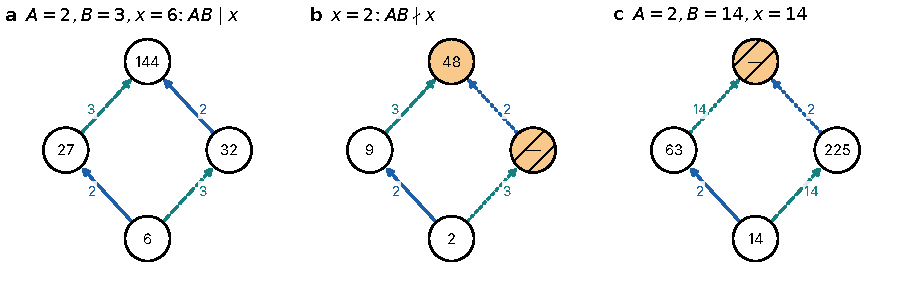
\includegraphics[width=\textwidth]{fig07_swap_diamonds}
\caption{\textbf{Legal and forbidden swap diamonds (exact).} Each panel shows the states (circles) reached from a state $x$ by the labels $A$ (solid blue edges) and $B$ (dashed teal edges); dotted edges and hatched orange nodes are inadmissible. (a) $A=2$, $B=3$, $x=6$: $AB\mid x$, the diamond closes at $144$. (b) $x=2$: $A=2$ is admissible but $B=3$ is not, so only one side exists. (c) $A=2$, $B=14$, $x=14$: both labels are admissible at $14$ but $AB=28\nmid14$, so after $2$ the label $14$ fails ($63$ is not divisible by $14$) and after $14$ the label $2$ fails. Theorem illustrated: \cref{prop:diamond}.}\label{fig:diamonds}
\end{figure}
\noindent The figure above is \cref{fig:diamonds}; its caption states the exactness of what is drawn.
\begin{theorem}[complete classification of $\{2,3,14\}$]\label{thm:2314}
The thresholds are $K=14$ for $(14,3,2),(2,3,14)$, $K=28$ for $(14,2,3),(2,14,3)$, and $K=21$ for $(3,14,2),(3,2,14)$. The number of swap classes of $\{2,3,14\}$ at the source $m$ is
\[
 \nu=\begin{cases}0&\text{if neither }14\text{ nor }21\text{ divides }m,\\ 2&\text{if }14\mid m\text{ and }\gcd(m/14,6)=1,\\ 1&\text{otherwise.}\end{cases}
\]
In particular, the two arrangements $(14,3,2)$ and $(2,3,14)$ lie in one class iff $28\mid m$ or $42\mid m$ (their connection thresholds), and from $m=14q$ there are two classes iff $\gcd(q,6)=1$. All admissible arrangements from $m$ end at $m\cdot2700/7$.
\end{theorem}
\begin{proof}
The thresholds were computed in \cref{ex:K}. Order the arrangements around the hexagon $\mathcal G(C)$ as $\sigma_0=(14,3,2)$, $\sigma_1=(3,14,2)$, $\sigma_2=(3,2,14)$, $\sigma_3=(2,3,14)$, $\sigma_4=(2,14,3)$, $\sigma_5=(14,2,3)$ (consecutive ones, and $\sigma_5,\sigma_0$, differ by an adjacent exchange). Then $\sigma_0,\sigma_3$ have threshold $14$ and are antipodal, $\sigma_1,\sigma_2$ have threshold $21$ and are adjacent, and $\sigma_4,\sigma_5$ have threshold $28$ and are adjacent. Every threshold is a multiple of $7$, so $7\mid m$ is necessary for any arrangement to be admissible. Now $\mathcal A(m)$ is the union of the pairs whose threshold divides $m$. If $14\nmid m$ then $28\nmid m$ and $\mathcal A(m)\subseteq\{\sigma_1,\sigma_2\}$, which is empty if $21\nmid m$ and one edge (one class) if $21\mid m$. If $14\mid m$ then $\sigma_0,\sigma_3\in\mathcal A(m)$; adding the $28$-pair when $28\mid m$ gives the path $\sigma_3\sigma_4\sigma_5\sigma_0$, adding the $21$-pair when $21\mid m$ gives the path $\sigma_0\sigma_1\sigma_2\sigma_3$; in either case the graph is connected, while with neither it is two isolated vertices. Finally $14\mid m$ and $21\nmid m$ and $28\nmid m$ means $14\mid m$, $3\nmid m$ and $m/14$ odd, i.e.\ $\gcd(m/14,6)=1$. The connection thresholds are $\lcm(14,28)=28$ and $\lcm(14,21)=42$. The common endpoint is $mR(2)R(3)R(14)=m\cdot\frac92\cdot\frac{16}3\cdot\frac{225}{14}=m\cdot\frac{2700}7$.
\end{proof}
\prov{CW-0348}{D-T10}{PROVED}{FULL}
\begin{corollary}[an infinite family of complete histories]\label{cor:family14}
Let $q\ge1$ be squarefree and coprime to $42$. Then $14q$ is squarefree, and the two complete histories $(14q;14,3,2)$ and $(14q;2,3,14)$, both ending at $5400q$, lie in different swap classes.
\end{corollary}
\begin{proof}
$14q$ is squarefree because $q$ is squarefree and coprime to $2\cdot7$; $\gcd(q,6)=1$ gives two classes by \cref{thm:2314}.
\end{proof}
\prov{CW-0342}{D-T5}{PROVED}{FULL}
\begin{figure}[tbp]\centering
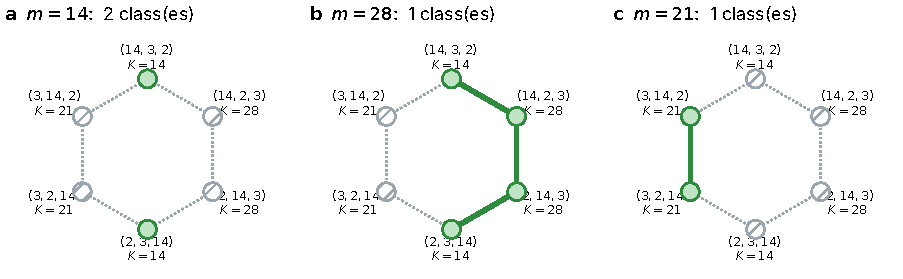
\includegraphics[width=\textwidth]{fig08_same_content_two_components}
\caption{\textbf{The same content in different swap components (exact).} The hexagon $\mathcal G(\{2,3,14\})$ with the threshold $K$ of each arrangement; admissible vertices at the source $m$ are shaded green and joined by thick solid green lines, inadmissible ones are hatched. (a) $m=14$: the antipodal pair $(14,3,2),(2,3,14)$, two classes, with the histories of \cref{ex:src14}. (b) $m=28$: the $28$-pair joins them, one class. (c) $m=21$: only the $21$-pair, one class. Theorem illustrated: \cref{thm:2314}.}\label{fig:hex}
\end{figure}
\noindent The figure above is \cref{fig:hex}; its caption states the exactness of what is drawn.
\begin{remark}
\Cref{thm:2314} relaxes a restriction of the earliest release: there the pair was shown for $q$ squarefree and coprime to $210$; the condition on the prime $5$ is unnecessary for the statement about fixed-source histories, as the proof shows (and $7\nmid q$ is needed only for squarefreeness of the source).
\end{remark}

\section{Feeding relations, factorisation and components}\label{sec:feeding}
\begin{definition}[feeding digraph, blocks]\label{def:feeding}
For labels $A\ne B$ say that $A$ \emph{feeds} $B$ if $\gcd(A+1,B)>1$ (a prime of $A+1$ divides $B$: running $A$ produces a resource that $B$ consumes). The \emph{feeding digraph} of a multiset $C$ has the distinct labels of $C$ as vertices and the pairs $(A,B)$ with $A$ feeding $B$ as edges. Its strongly connected components are the \emph{blocks}; the condensation is acyclic, so the blocks can be listed in a \emph{topological order}, feeders first: if $A$ feeds $B$ then the block of $A$ is not later than the block of $B$.
\end{definition}
\begin{lemma}[NF: non-feeding pairs commute]\label{lem:NF}
If $x$ does not feed $y$ and $(x,y)$ is admissible from a state $s$, then $(y,x)$ is admissible from $s$. Consequently, for $x\neq y$ with $x$ not feeding $y$, an adjacent pair $(x,y)$ in an admissible word can always be exchanged to $(y,x)$.
\end{lemma}
\begin{proof}
$\gcd(x+1,y)=1$ gives $\gcd(y,(x+1)^2)=1$, so $K((x,y))=xy$ by \cref{prop:diamond}(a). Also $K((y,x))=xy/\gcd(x,(y+1)^2)$ divides $xy$. Hence $K((y,x))\mid K((x,y))\mid s$.
\end{proof}
\prov{CW-0350}{NF}{PROVED}{FULL}
\begin{theorem}[block factorisation]\label{thm:F2}
Let $C$ be a multiset (repeated labels allowed) with blocks $B_1,\dots,B_r$ in topological order, $C_i$ the sub-multiset of $C$ on $B_i$, and $m_0=m$, $m_i=m_{i-1}R(C_i)$. Then
\[
 \nu(C,m)=\prod_{i=1}^r\nu(C_i,m_{i-1}),
\]
where $\nu(C_i,y)$ is read as $0$ if $y$ is not an integer. In particular $\nu(C,m)=0$ as soon as one factor is $0$.
\end{theorem}
\begin{proof}
\emph{Sorting.} Let $w$ be admissible from $m$ and let $x,y$ be adjacent letters of $w$ with $x$ in a later block than $y$. Then $x$ does not feed $y$ (an edge $x\to y$ would put the block of $x$ no later than that of $y$), so by \cref{lem:NF} exchanging them is a legal swap. A stable bubble sort by block index reaches the block-sorted word $u_1\cdots u_r$, where $u_i$ is the subword of $w$ on $C_i$, by legal swaps of letters of different blocks; so $u_1\cdots u_r$ is admissible, hence each $u_i$ is admissible from $m_{i-1}$ (the state after $u_1\cdots u_{i-1}$ is $m_{i-1}$ whatever the orders inside the $u_j$).
\emph{Invariant.} Let $\pi_i(w)$ be the subword of $w$ on $C_i$. A legal swap of two letters from different blocks leaves every $\pi_i$ unchanged. A legal swap of two letters of the same block $B_i$ changes only $\pi_i$, by one exchange of adjacent distinct letters (the letters are adjacent in $w$, hence in $\pi_i$); sorting $w$ and the swapped word gives two admissible block-sorted words that differ by this exchange inside the $i$-th segment, so the exchange is a legal swap in $\mathrm{Sw}(C_i,m_{i-1})$. Therefore the tuple of classes $([\pi_1(w)],\dots,[\pi_r(w)])$ is constant on swap classes of $C$ at $m$.
\emph{Bijection.} The map $w\mapsto([\pi_i(w)])_i$ from swap classes to $\prod_i\{\text{classes of }\mathrm{Sw}(C_i,m_{i-1})\}$ is onto: concatenating admissible block words $v_i$ from $m_{i-1}$ gives an admissible word, because the entry state of block $i$ is $m_{i-1}$ whatever was chosen before. It is injective: two words with the same tuple are connected by sorting both and then moving inside each block along a path of $\mathrm{Sw}(C_i,m_{i-1})$; each such step is a legal swap of the whole word, since the state before block $i$ is $m_{i-1}$ in both.
\end{proof}
\prov{CW-0351}{F2}{PROVED}{FULL}
\begin{corollary}[acyclic feeding digraph]\label{cor:F1}
If every block is a single label (the feeding digraph is acyclic), then $\nu(C,m)\le1$ for every $m$. Moreover for the block-sorted word $\tau$ one has $K(\tau)\mid K(w)$ for every arrangement $w$, so $K(\tau)$ is the universal minimal threshold, and $\mathcal A(m)$ is a lower set of the weak order determined by $\tau$ (\cref{sec:feasible}).
\end{corollary}
\begin{proof}
Each $C_i$ is a power of one letter and has one arrangement, so each factor of \cref{thm:F2} is $0$ or $1$. For the second claim, a legal exchange of an inverted pair (relative to $\tau$) turns an admissible word $w$ into an admissible $w'$ (\cref{lem:NF}); applying it at the source $m=K(w)$ shows $K(w')\mid K(w)$, and bubble sort ends at $\tau$.
\end{proof}
\prov{CW-0351}{F2}{PROVED}{FULL}
\begin{remark}
An acyclic feeding digraph is a \emph{sufficient} condition for connectivity at every source; it is not necessary (a strongly connected content may never split; see \cref{ex:sccnever}). Conversely, a split needs a block with at least $3$ labels: a block with at most two distinct labels, each once, has at most two arrangements, which are adjacent, so for contents of distinct labels such a block never splits.
\end{remark}

\subsection{Hub descent}
\begin{proposition}[hub-descent criterion]\label{prop:hub}
Call an arrangement $h$ of $C$ a \emph{hub} if $K(h)\mid K(w)$ for all arrangements $w$ and every $w$ has a path $w=v_0,v_1,\dots,v_s=h$ in $\mathcal G(C)$ with $K(v_{i+1})\mid K(v_i)$. If a hub exists then $\nu(C,m)\le1$ for all $m$.
\end{proposition}
\begin{proof}
If $w\in\mathcal A(m)$ then $K(h)\mid K(w)\mid m$ and every $v_i$ on the descent path has $K(v_i)\mid K(w)\mid m$, so $w$ is joined to $h$ inside $\mathrm{Sw}(C,m)$.
\end{proof}
\prov{CW-0352}{Hub-descent}{PROVED}{FULL}
The criterion is sufficient but not necessary. \emph{Finite-exact census:} over the $4060$ contents of three distinct labels in $\{1,\dots,30\}$, $3408$ have a hub and never split, none has a hub and a split, $525$ have neither a hub nor a split, and $127$ split (all without a hub); for four distinct labels in $\{1,\dots,14\}$ the counts are $773/0/125/103$.
\prov{CW-0353}{CONNECTIVITY:Census-on-three-labels-FINITE}{FINITE-EXACT}{FINITE}

\subsection{Three distinct labels}
For a multiset $S$ of labels, $\kappa(S)$ is as in \cref{sec:threshold}. For three distinct labels the arrangement graph is the hexagon.
\begin{theorem}[exact classification of three distinct labels]\label{thm:T3}
Let $C=\{x,y,z\}$ consist of three distinct labels. The swap graph of $C$ at $m$ is disconnected if and only if there is a labelling $(a,b,c)$ of $C$ such that
\[
 a\mid m,\quad c\mid m,\quad \kappa\{a,b\}\mid m,\quad \kappa\{b,c\}\mid m,\quad \kappa\{a,b,c\}\mid m,\qquad b\nmid m,\quad \kappa\{a,c\}\nmid m .
\]
In that case $\mathcal A(m)=\{(a,b,c),(c,b,a)\}$, an antipodal pair of the hexagon, and $\nu(C,m)=2$. A content has a split source iff for some labelling $L=\lcm(a,c,\kappa\{a,b\},\kappa\{b,c\},\kappa\{a,b,c\})$ is divisible by neither $b$ nor $\kappa\{a,c\}$; the split sources of that labelling are the multiples $m$ of $L$ with $b\nmid m$ and $\kappa\{a,c\}\nmid m$.
\end{theorem}
\begin{proof}
($\Leftarrow$) By \cref{cor:P} the prefix multisets of $(a,b,c)$ are $\{a\},\{a,b\},C$ and of $(c,b,a)$ are $\{c\},\{c,b\},C$, all feasible by hypothesis ($\kappa\{a\}=a$, $\kappa\{c\}=c$). The words $(a,c,b)$ and $(c,a,b)$ have the prefix multiset $\{a,c\}$ and $(b,a,c)$, $(b,c,a)$ have $\{b\}$; both are infeasible by hypothesis ($\kappa\{b\}=b$). So $\mathcal A(m)$ is the antipodal pair, which is disconnected.
($\Rightarrow$) Let $\mathcal A(m)$ be disconnected and $u,w$ in different components. If $u,w$ were at distance $2$ in the hexagon, their unique common neighbour $v$ arises from $u$ and from $w$ by exchanges at different positions, so each prefix multiset of $v$ is a prefix multiset of $u$ or of $w$; by \cref{cor:P} $K(v)\mid\lcm(K(u),K(w))\mid m$, so $v\in\mathcal A(m)$ and $u,w$ would be connected. Hence any two vertices in different components are antipodal. A vertex has a unique antipode, so no component contains two vertices (they would both be antipodal to every vertex of another component) and there are at most two components. Thus $\mathcal A(m)=\{w,w^{\mathrm{rev}}\}$; write $w=(a,b,c)$. Its prefix multisets $\{a\},\{a,b\},\{c\},\{c,b\},C$ are feasible, which gives the five divisibilities; the four other arrangements are inadmissible, and $(a,c,b)$ (resp.\ $(b,a,c)$) has $\{a,c\}$ (resp.\ $\{b\}$) as its only prefix multiset not among the feasible ones, so $\kappa\{a,c\}\nmid m$ and $b\nmid m$. The last statements follow by taking the least $m$ satisfying the divisibilities.
\end{proof}
\prov{CW-0354}{T3}{PROVED}{FULL}
\begin{remark}
The mechanism in words: $b$ alone is infeasible (it consumes something that only $a$ or $c$ produces) and $\{a,c\}$ together is infeasible (they consume something only $b$ produces); everything else is feasible. The two histories can only be run ``through $b$'' from the ends and cannot be exchanged into each other.
\end{remark}

\subsection{The family \texorpdfstring{$\{2,3,N\}$}{{2,3,N}}}
\begin{theorem}[the family $\{2,3,N\}$]\label{thm:23N}
Let $N\ge4$, $N\ne2,3$, and $C=\{2,3,N\}$.
\begin{enumerate}[label=(\alph*),itemsep=1pt]
\item The feeding digraph of $C$ is strongly connected iff $N\equiv2$ or $3\pmod 6$ (then $N\ge8$). Otherwise its blocks are $\{2,3\}$ and $\{N\}$ and $\nu(C,m)\le1$ for every $m$.
\item If $N\equiv2,3\pmod6$ then $\nu(C,m)=2$ iff $m=Nt$ with $\gcd(t,6)=1$, and $\nu(C,m)\le1$ otherwise. In particular $C$ has a split source iff $N\equiv2,3\pmod6$, and then the minimal split source is $N$ itself, where $\mathcal A(N)$ is $\{(2,3,N),(N,3,2)\}$ for $N\equiv2$ and $\{(N,2,3),(3,2,N)\}$ for $N\equiv3\pmod 6$.
\end{enumerate}
\end{theorem}
\begin{proof}
(a) $2$ and $3$ feed each other ($\gcd(3,3)=3$, $\gcd(4,2)=2$). $N$ feeds $2$ iff $N$ is odd; $N$ feeds $3$ iff $3\mid N+1$; $2$ feeds $N$ iff $3\mid N$; $3$ feeds $N$ iff $N$ is even. So $N$ lies in the block of $\{2,3\}$ iff ($N$ odd or $N\equiv2\bmod3$) and ($N$ even or $3\mid N$), which is $N\equiv2,3\pmod 6$ by inspecting the six residues. Otherwise the blocks $\{2,3\}$ and $\{N\}$ each have at most one arrangement up to an adjacent exchange, so every factor of \cref{thm:F2} is $\le1$.
(b) Let $N\equiv2\pmod 6$: $N$ is even, $3\nmid N$, $3\mid N+1$; write $a=v_2(N)\ge1$, $N=2^aR$ with $R$ odd and prime to $3$, and $c=v_3(N+1)\ge1$. Direct computation of $\Delta$ gives $\kappa\{2\}=2$, $\kappa\{3\}=3$, $\kappa\{N\}=N$, $\kappa\{2,3\}=1$ (as $R(2)R(3)=24$), $\kappa\{2,N\}=2^{a+1}R=2N$, $\kappa\{3,N\}=2^{\max(0,a-4)}R$ and $\kappa\{2,3,N\}=2^{\max(0,a-3)}R$ (for the primes $q\ge5$ only the consumption $v_q(N)$ matters, and $3$ is produced by $2$, $N$ and consumed only by $3$). By \cref{cor:P}, $K(2,3,N)=2^{\max(1,a-3)}R$ and $K(N,3,2)=N$ both divide $N$, while $K(2,N,3)$, $K(N,2,3)$ are multiples of $2N$ and $K(3,\cdot,\cdot)$ of $3$, none of which divides $N$. So $\mathcal A(N)=\{(2,3,N),(N,3,2)\}$, antipodal, $\nu(C,N)=2$. For general $m$ use \cref{thm:T3}: the middle label $b$ must not divide $m$ while the two ends do. If $b=2$ then $2\nmid m$, but $N$ is an end, so $2\mid N\mid m$, a contradiction. If $b=N$ then one of $\kappa\{a,b\},\kappa\{b,c\}$ is $\kappa\{2,N\}=2N$ and must divide $m$, forcing $N\mid m$, a contradiction. So $b=3$, the ends are $2,N$, and the conditions of \cref{thm:T3} read: $N\mid m$ (all of $\kappa\{3,N\},\kappa\{2,3,N\}$ divide $N$), $3\nmid m$ and $2N\nmid m$; with $m=Nt$ these say $3\nmid t$ and $t$ odd.
For $N\equiv3\pmod6$ the roles of $2$ and $3$ are exchanged: $N$ is odd, $N=3^bR$ with $\gcd(R,6)=1$, $b\ge1$, $c=v_2(N+1)\ge1$, $\kappa\{3,N\}=3^{b+1}R=3N$, $\kappa\{2,N\}=3^{\max(0,b-2)}R$, $\kappa\{2,3,N\}=3^{\max(0,b-1)}R$, $\kappa\{2,3\}=1$; $\mathcal A(N)=\{(N,2,3),(3,2,N)\}$, and the same argument forces the middle label to be $2$ and gives $\nu(C,m)=2$ iff $N\mid m$, $2\nmid m$, $3N\nmid m$, i.e.\ $m=Nt$, $\gcd(t,6)=1$. In both cases $N\ge8$ is automatic since $N\ge4$ and $N\notin\{2,3\}$ and $N\equiv2,3\pmod 6$.
\end{proof}
\begin{remark}[status relative to the source]
The source release proves the arithmetic of the family and records only a finite-exact range ($4\le N\le400$) for the converse. Part (a) together with \cref{thm:F2} and the argument of (b) prove the converse for all $N\ge4$; the finite range is corroboration.
\end{remark}
\prov{CW-0347}{D-T9}{MIXED}{SPLIT}\prov{CW-0355}{OBSTRUCTIONS:Parameter-family-2-3-N-PROV}{PROVED}{FULL}
\begin{figure}[tbp]\centering
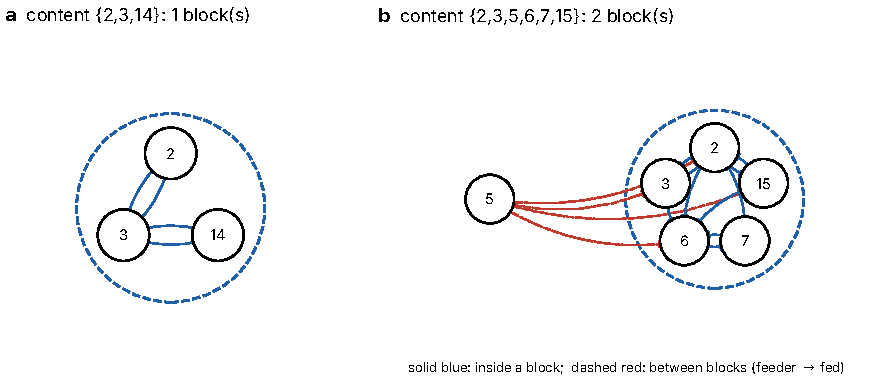
\includegraphics[width=\textwidth]{fig09_feeding_blocks}
\caption{\textbf{Feeding digraphs and blocks (exact).} Dashed blue circles are strongly connected blocks; solid blue arrows are feeding edges inside a block and dashed red arrows are feeding edges between blocks (feeder to fed). (a) $\{2,3,14\}$: one block ($3$ feeds $14$ and $14$ feeds $3$; $14$ does not feed $2$ or conversely). (b) $\{2,3,5,6,7,15\}$: the label $5$ is a block of its own feeding the block $\{2,3,6,7,15\}$. Theorems illustrated: \cref{thm:F2}, \cref{cor:F1}.}\label{fig:feeding}
\end{figure}
\noindent The figure above is \cref{fig:feeding}; its caption states the exactness of what is drawn.
\begin{figure}[tbp]\centering
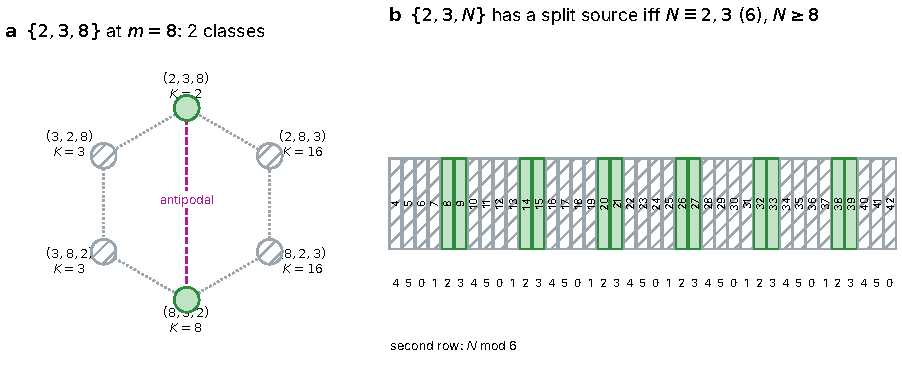
\includegraphics[width=\textwidth]{fig10_three_label_split}
\caption{\textbf{Three-label split and the antipodal orderings (exact; the strip is exact in the range shown).} (a) The hexagon of $\{2,3,8\}$ at $m=8$ with the threshold $K$ of each arrangement: only the antipodal pair $(2,3,8),(8,3,2)$ is admissible (two classes). (b) The integers $N=4,\dots,42$ with residues mod $6$: shaded cells are those for which $\{2,3,N\}$ has a split source, namely $N\equiv2,3\pmod 6$ with $N\ge8$. Theorems illustrated: \cref{thm:T3}, \cref{thm:23N}.}\label{fig:split}
\end{figure}
\noindent The figure above is \cref{fig:split}; its caption states the exactness of what is drawn.
\begin{example}[strongly connected, never split]\label{ex:sccnever}
The contents $\{2,4,15\}$, $\{2,5,9\}$ and $\{2,6,7\}$ have strongly connected feeding digraphs and $\nu\le1$ at every source in the lcm-closure of their thresholds. Strong connectivity of the feeding digraph is therefore necessary but not sufficient for a split.
\end{example}
\begin{proposition}[finite-exact: all three-label splits are antipodal]\label{prop:census3}
Among the $\binom{30}{3}=4060$ contents of three distinct labels in $\{1,\dots,30\}$, exactly $257$ have a strongly connected feeding digraph and exactly $127$ have a split source; each split content is strongly connected, so $130$ strongly connected contents never split. For each of the $4060$ contents and every source in the lcm-closure of its thresholds, the criterion of \cref{thm:T3} agrees with the direct class count (no violation). \stat{finite-exact}.
\end{proposition}
\prov{CW-0349}{THEOREMS\_V002:Census-FINITE-EXACT-results}{FINITE-EXACT}{FINITE}

\section{Feasible-subset geometry and topological obstructions}\label{sec:feasible}
Throughout this section $C$ is a set of $k\ge3$ \emph{distinct} labels (repeated labels need a different construction, \cref{prob:repeated}).
\subsection{Feasible subsets and maximal chains}
By \cref{cor:P} an arrangement $w$ is admissible from $m$ iff every prefix set of $w$ is feasible at $m$. For distinct labels the admissible histories of content $C$ are therefore exactly the \emph{maximal chains} $\emptyset\subset S_1\subset\cdots\subset S_k=C$ of feasible subsets ($S_j$ the set of the first $j$ letters). A set $S\subseteq C$ is \emph{infeasible} at $m$ iff for some prime $p$,
\[
 \sum_{x\in S}\Delta_p(x)<-v_p(m),
\]
a knapsack-type threshold: $S$ consumes more of the resource $p$ than $m$ supplies plus what its members themselves produce. The whole route theory is a theory of the family of infeasible proper subsets (\cref{fig:lattice}). The set $C$ itself is feasible whenever $\mathcal A(m)\neq\emptyset$.
\begin{figure}[tbp]\centering
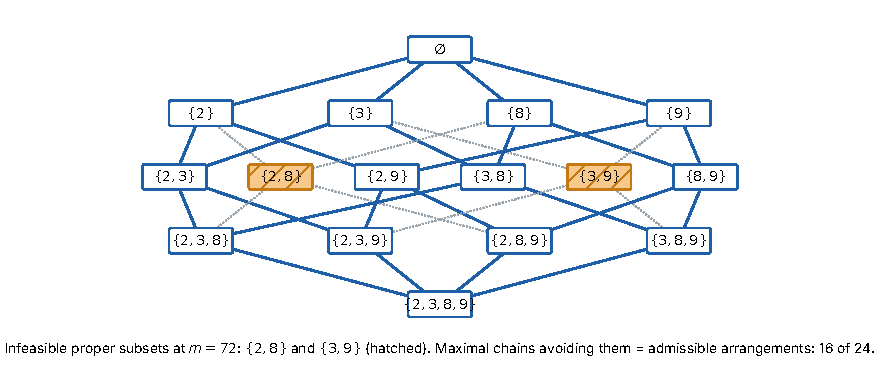
\includegraphics[width=\textwidth]{fig11_feasible_subsets}
\caption{\textbf{Feasible-subset diagram of $\{2,3,8,9\}$ at $m=72$ (exact).} The Boolean lattice of subsets; the two infeasible proper subsets $\{2,8\}$ and $\{3,9\}$ are hatched orange, and the edges at them are dotted grey. The maximal chains $\emptyset\subset\cdots\subset C$ that avoid them are the admissible arrangements: $16$ of the $24$. Theorem illustrated: \cref{cor:P}, \cref{thm:sphere}.}\label{fig:lattice}
\end{figure}

\subsection{The route complexes}
The permutohedron $P_k$ is the convex hull of the points $(\sigma(1),\dots,\sigma(k))\in\mathbb R^k$, $\sigma$ a permutation; it is a simple $(k-1)$-polytope whose boundary is homeomorphic to $S^{k-2}$, and its faces correspond to the ordered set partitions $(B_1|\cdots|B_j)$ of the labels, with dimension $k-j$ and vertex set the arrangements that list $B_1$ first (in any order), then $B_2,\dots$ (see Ziegler~\cite[Example~0.10]{Ziegler1995}). The vertices are the arrangements and the edges are the exchanges of adjacent letters.
\begin{definition}[route complexes]\label{def:routecx}
For a set $\mathcal A$ of arrangements, the \emph{permutohedral route complex} $K_{\mathcal A}$ is the full subcomplex of the face complex of $P_k$ on the vertex set $\mathcal A$: a face is kept iff all its vertices lie in $\mathcal A$. The \emph{cubical route complex} $Q_{\mathcal A}$ is the subcomplex of faces all of whose blocks have size $\le2$ (products of edges): its vertices are the admissible histories, its edges the legal swaps, and its squares and cubes the sets of independent swaps (\cref{lem:indep}). We write $K_m=K_{\mathcal A(m)}$ and $Q_m$. Homology is over $\mathbb F_2$ unless stated. The $1$-skeleton of either complex is the swap graph, so $\beta_0$ counts swap classes. A hexagon (braid relation $xyz\leftrightarrow zyx$) is a $2$-face of $K_m$ iff all six arrangements of the three letters are admissible, and is \emph{never} a cell of $Q_m$.
\end{definition}
\begin{remark}
Faces of $P_k$ containing a given vertex $v$ correspond to subsets of the $k-1$ adjacent position pairs of $v$ (the blocks are the maximal intervals joined by the chosen pairs); this is the simplicity of $P_k$ and is used in \cref{thm:lower}.
\end{remark}

\subsection{Alexander duality}
Write $\mathcal R=\mathfrak S_k\setminus\mathcal A$ for the set of non-admissible arrangements and $\mathcal N(\mathcal R)$ for the simplicial complex on $\mathcal R$ whose simplices are the subsets of $\mathcal R$ contained in a common proper face of $P_k$.
The nerve theorem and Alexander duality used below are in~\cite{Hatcher2002}; the permutohedron is described in~\cite{Ziegler1995}.
\begin{theorem}[duality for route complexes]\label{thm:dual}
Let $\emptyset\ne\mathcal A\ne\mathfrak S_k$. Then $K_{\mathcal A}\subset\partial P_k\cong S^{k-2}$ and, over $\mathbb F_2$, for all $i$
\[
 \dim\tilde H_i(K_{\mathcal A})=\dim\tilde H^{\,k-3-i}\bigl(\mathcal N(\mathcal R)\bigr).
\]
Two vertices of $\mathcal R$ lie in a common proper face iff they share a proper prefix set; hence $\mathcal N(\mathcal R)$ has the connected components of the graph on $\mathcal R$ joined by ``share a proper prefix set''. Consequently $\tilde\beta_{k-2}(K_{\mathcal A})=0$ and $\tilde\beta_{k-3}(K_{\mathcal A})=c(\mathcal R)-1$, where $c(\mathcal R)$ is the number of such components. In particular for $k=3$, $\tilde\beta_1=0$; for $k=4$, $\beta_2=0$ and $\beta_1=c(\mathcal R)-1$; for $k=5$, $\beta_3=0$ and $\beta_2=c(\mathcal R)-1$.
\end{theorem}
\begin{proof}
$K_{\mathcal A}$ is a proper nonempty subcomplex of the sphere $\partial P_k$ (a vertex of $\mathcal R$ lies outside it). A point $x\in\partial P_k$ lies in the relative interior of a unique face $F$, and $x\in K_{\mathcal A}$ iff all vertices of $F$ lie in $\mathcal A$. Hence the complement of $K_{\mathcal A}$ is the union, over $v\in\mathcal R$, of the open stars $\mathrm{st}(v)$ (the union of the relative interiors of the faces containing $v$). Each open star is open in $\partial P_k$ (its complement is the union of the faces not containing $v$) and contractible (it is star-shaped from $v$). For a family $v_1,\dots,v_n$ the intersection $\bigcap\mathrm{st}(v_i)$ is the union of the relative interiors of the faces containing all $v_i$; these are the faces containing the smallest face $\Phi$ containing all $v_i$ (an intersection of faces is a face), so the intersection is $\mathrm{st}(\Phi)$, which is contractible, provided $\Phi$ is a proper face, and it is empty otherwise (there is no proper face containing all $v_i$). By the nerve theorem for open covers~\cite[Cor.~4G.3]{Hatcher2002} the complement of $K_{\mathcal A}$ is homotopy equivalent to the nerve of this cover, which is $\mathcal N(\mathcal R)$. Alexander duality~\cite[Prop.~3.46]{Hatcher2002} applied to the compact, locally contractible, nonempty proper subspace $K_{\mathcal A}$ of $S^{k-2}$ gives $\tilde H_j(S^{k-2}\setminus K_{\mathcal A})\cong\tilde H^{k-3-j}(K_{\mathcal A})$; over a field $\tilde H^q$ and $\tilde H_q$ of a finite complex have equal dimension, which gives the displayed equality after exchanging the roles of the two sides. Two vertices lie in a common proper face iff they lie in a face $(B_1|\cdots|B_j)$ with $j\ge2$, i.e.\ iff they both begin with the proper subset $B_1$, i.e.\ share a proper prefix set. Finally $\tilde H^{-1}$ of a nonempty complex vanishes (this gives $\tilde\beta_{k-2}=0$) and $\tilde\beta^0$ counts components minus one.
\end{proof}
\prov{CW-0359}{T-DUAL}{PROVED}{FULL}
\emph{Check.} The identity $\beta_{k-3}=c(\mathcal R)-1$ (and $\beta_{k-2}=0$) was verified against independent direct homology computations for $1772$ complexes with $k=4,5$ (a sample of contents with labels $\le14$, resp.\ $\le11$, and all sources in the lcm-closure), with no violation (\texttt{results/RESULTS\_II\_part3.json}). \stat{finite-exact} corroboration.

\subsection{Lower sets are contractible}
Fix a total order $\tau$ on the labels. The \emph{weak order} on arrangements is $u\le v$ iff the inversion set of $u$ (pairs ordered differently from $\tau$) is contained in that of $v$; its minimum is the $\tau$-sorted word $b$ and its maximum the reverse. A set $\mathcal A$ is a \emph{lower set} if it is closed under replacing an adjacent inverted pair by the non-inverted one.
\begin{theorem}[lower sets]\label{thm:lower}
If $\mathcal A$ is a nonempty lower set of the weak order, then $K_{\mathcal A}$ is contractible. Consequently, if the feeding digraph of $C$ is acyclic, then $K_m$ is empty or contractible for every source $m$.
\end{theorem}
\begin{proof}
If $\mathcal A=\mathfrak S_k$ then $K_{\mathcal A}$ is the single cell $P_k$; otherwise $b\in\mathcal A$ since $\mathcal A$ is nonempty and a lower set. Induct on $|\mathcal A|$; for $\mathcal A=\{b\}$ the complex is a point. Let $v\ne b$ be maximal in $\mathcal A$. Faces of $P_k$ through $v$ correspond to subsets $J$ of the $k-1$ adjacent position pairs of $v$. If $J$ contains an ascent of $v$ (an adjacent pair in $\tau$-order), the face contains the neighbour of $v$ obtained by exchanging it, which has one more inversion and is not in $\mathcal A$ by maximality. If $J$ consists of descents only, each block of the face is a segment of a decreasing run, so all vertices of the face are obtained from $v$ by sorting inside blocks and are $\le v$, hence in $\mathcal A$. So the faces of $K_{\mathcal A}$ through $v$ correspond to the subsets of $\mathrm{Desc}(v)$, nonempty because $v\ne b$: the link of $v$ in $K_{\mathcal A}$ is a full simplex $L$ (contractible), and the closed star of $v$ is a cone over it. Then $K_{\mathcal A}=K_{\mathcal A\setminus\{v\}}\cup\mathrm{star}(v)$ with $K_{\mathcal A\setminus\{v\}}\cap\mathrm{star}(v)=L$; gluing a cone along its contractible base does not change the homotopy type, so $K_{\mathcal A}\simeq K_{\mathcal A\setminus\{v\}}$, and $\mathcal A\setminus\{v\}$ is again a nonempty lower set. For the consequence: choose $\tau$ so that feeders come first; if $x$ does not feed $y$ and $x$ is placed after $y$ in $\tau$-order... precisely, an inverted adjacent pair $(x,y)$ ($x$ after $y$ in $\tau$) has $x$ not feeding $y$ because all feeding edges go forward in $\tau$; by \cref{lem:NF} replacing it by $(y,x)$ keeps an admissible word admissible. So $\mathcal A(m)$ is a lower set.
\end{proof}
\prov{CW-0360}{T-LOWER}{PROVED}{FULL}
\emph{Check.} For $303$ nonempty route complexes of contents of four distinct labels with acyclic feeding digraph (labels $\le15$, sources among the thresholds), every $K_m$ has Betti vector $(1,0,0,0)$; no violation. \stat{finite-exact} corroboration.

\subsection{Complementary pairs and spheres}
\begin{theorem}[complementary-pair deadlock]\label{thm:sphere}
Let $C=E\sqcup O$ be a partition into nonempty sets and suppose the infeasible proper subsets of $C$ at $m$ are exactly $E$ and $O$. Then $K_m$ has the $\mathbb F_2$-homology of the sphere $S^{k-3}$: $\beta_0=1$ and $\beta_{k-3}=1$ with all other Betti numbers zero (for $k=3$: two points, $\beta_0=2$, the antipodal pair of \cref{thm:T3}).
\end{theorem}
\begin{proof}
The non-admissible arrangements are those having $E$ or $O$ as a prefix set, i.e.\ $\mathcal R=F_{E|O}\sqcup F_{O|E}$, the vertex sets of two facets. A vertex $v$ of the first facet and a vertex $w$ of the second have no common proper prefix set: a proper prefix set of $v$ of size $s\le|E|$ is a subset of $E$ and for $s\ge|E|$ contains $E$, symmetrically for $w$ with $O$; equality of such sets is impossible unless the set is $C$ (the sets would have to lie in both $E$ and $O$, or contain both). Hence $\mathcal N(\mathcal R)$ has exactly two components, each a full simplex (all vertices of a facet lie in a common proper face). So $\tilde H^0(\mathcal N(\mathcal R))$ has rank one and all other reduced groups vanish, and \cref{thm:dual} gives $\tilde\beta_{k-3}=1$ and all other reduced Betti numbers $0$.
\end{proof}
\prov{CW-0361}{T-SPHERE}{PROVED}{FULL}
\begin{remark}[scope]
The homotopy type of $K_m$ is not determined by this argument: it is a statement about $\mathbb F_2$-homology. (That $K_m$ is homotopy equivalent to $S^{k-3}$ would follow if the union of the open stars of the vertices of each facet were an open ball in the sphere, which is plausible but not proved here.) The arithmetic hypothesis (infeasible subsets exactly $E$ and $O$) is a condition on $(C,m)$ that is checked case by case, not a theorem.
\end{remark}
\begin{proposition}[arithmetic realisation; finite-exact]\label{prop:realise}
Let $X$ be a set of labels $n\equiv2,3\pmod6$, $n\ge8$, $C=\{2,3\}\cup X$ and $m=\prod_{x\in X}x$. For all $X\subseteq\{8,9,14,15,20,21\}$ with $1\le|X|\le3$ ($41$ contents) the infeasible proper subsets of $C$ at $m$ are exactly $E=\{x\in C:x\equiv2\bmod 6\}$ and $O=\{x\in C:x\equiv3\bmod6\}$, and the Betti vector of $K_m$ is that of $S^{k-3}$. \stat{finite-exact}.
\end{proposition}
Two instances are the examples that drive the manuscript.
\begin{example}[loop: $\{2,3,8,9\}$ at $72$]\label{ex:loop}
$E=\{2,8\}$, $O=\{3,9\}$, $m=8\cdot9=72$. Of the $24$ arrangements $16$ are admissible, the swap graph is connected, and $K_{72}$ has $f$-vector $(16,20,4)$ (four $2$-faces) and Betti vector $(1,1,0,0)$: a loop of legal swaps that is not filled. The cubical complex $Q_{72}$ has the same $f$-vector and the same Betti vector. The loop is invisible to the connectivity classification (\cref{fig:lattice}, \cref{fig:loop}).
\end{example}
\begin{example}[void: $\{2,3,8,9,14\}$ at $1008$]\label{ex:void}
$E=\{2,8,14\}$, $O=\{3,9\}$, $m=8\cdot9\cdot14=1008$. There are $96$ admissible arrangements out of $120$; $K_{1008}$ has $f$-vector $(96,180,98,12)$ and Betti vector $(1,0,1,0,0)$: a $2$-dimensional void. The cubical complex $Q_{1008}$ has $f$-vector $(96,180,66)$ and Betti vector $(1,19,0,0,0)$: nineteen loops and no void, so the genuine obstruction is seen only after the braid hexagons are filled (\cref{fig:void}).
\end{example}
\begin{figure}[tbp]\centering
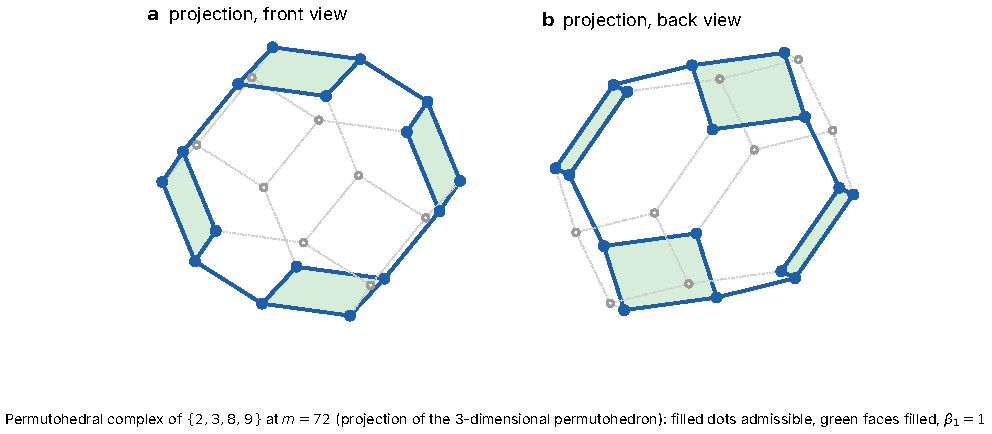
\includegraphics[width=\textwidth]{fig12_four_label_H1}
\caption{\textbf{The permutohedral route complex of $\{2,3,8,9\}$ at $m=72$ (exact; projection of a $3$-dimensional polytope to the plane, front and back views).} Filled blue dots are admissible arrangements, hollow dots are inadmissible; solid blue lines are legal swaps and dotted grey lines are non-legal exchanges; green faces are the four $2$-faces (squares and hexagons) all of whose vertices are admissible. The unfilled cycle of legal swaps is the generator of $H_1=\mathbb F_2$. The picture is a projection; the object is the $3$-dimensional permutohedron's boundary $S^2$. Theorems illustrated: \cref{thm:sphere}, \cref{ex:loop}.}\label{fig:loop}
\end{figure}
\begin{figure}[tbp]\centering
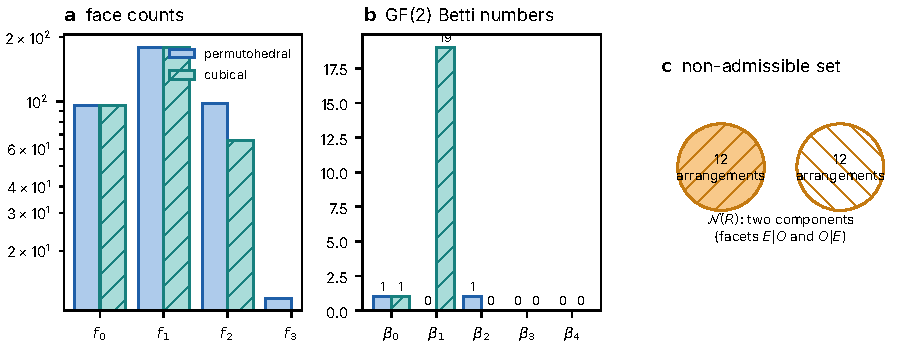
\includegraphics[width=\textwidth]{fig13_five_label_H2}
\caption{\textbf{The void of $\{2,3,8,9,14\}$ at $m=1008$ (exact; incidence data, not a drawing of the $4$-dimensional polytope).} (a) Face counts of the permutohedral complex $K_{1008}$ and of the cubical complex $Q_{1008}$ ($f_0,\dots,f_3$; logarithmic scale). (b) $\mathbb F_2$-Betti numbers: $(1,0,1,0,0)$ for $K_{1008}$ (blue, plain) and $(1,19,0,0,0)$ for $Q_{1008}$ (teal, hatched). (c) The non-admissible set $\mathcal R$ has $24$ arrangements in two components of $\mathcal N(\mathcal R)$ ($12$ and $12$, the facets $E|O$ and $O|E$), whence $\beta_2=2-1=1$ by \cref{thm:dual}. Theorems illustrated: \cref{thm:dual}, \cref{thm:sphere}, \cref{ex:void}.}\label{fig:void}
\end{figure}
\begin{proposition}[cubical versus permutohedral; finite-exact]\label{prop:cubperm}
For the full sets of arrangements ($P(C)\mid m$) of $k=3,4,5$ distinct labels, $K_m$ is a single cell (contractible), while $Q_m$ has Betti vectors $(1,1)$, $(1,7)$, $(1,31)$ respectively, computed here for $C=\{2,3,5\}$, $\{2,3,5,7\}$, $\{2,3,5,7,11\}$ at $m=P(C)$. So a cube-only complex reports loops that are mere braid relations. For $\{2,3,8,9\}$ at $72$ the two complexes agree (\cref{ex:loop}); for $\{2,3,8,9,14\}$ at $1008$ they differ in the way stated in \cref{ex:void}.
\end{proposition}
\prov{CW-0362}{ROUTE\_TOPOLOGY:Cubical-versus-permutohedral}{FINITE-EXACT}{FINITE}

\subsection{Loop family and census}
\begin{proposition}[loop family; finite-exact]\label{prop:loopfam}
For $8\le N<M<40$ with $N,M\equiv2,3\pmod 6$, the content $\{2,3,N,M\}$ has $\beta_1(K_{NM})>0$ (computed here for all such pairs). The programme's records state the converse over $4\le N<M\le60$ (a first Betti number appears at some source only if $N,M\ge8$ and $N,M\equiv2,3\bmod6$); this converse was not re-run here and is \stat{cited}.
\end{proposition}
\begin{proposition}[census; cited]\label{prop:census}
The programme's census over all sources in the lcm-closure records, for $k=3$ (labels $\le30$): $16\,378$ (content, source) pairs, Betti $(1,0,0)$ for $16\,251$ and $(2,0,0)$ for $127$; for $k=4$ (labels $\le18$): $27\,751$ pairs, of which $27\,321$ contractible, $16$ with $(1,1,0,0)$, $405$ with $(2,0,0,0)$, $7$ with $(3,0,0,0)$, $2$ with $(4,0,0,0)$; for $k=5$ (labels $\le11$): $8\,884$ pairs, $8\,617$ contractible, $21$ with $(1,1,0,0,0)$, $235$ with $(2,0,0,0,0)$, $11$ with $(3,0,0,0,0)$. No $\beta_i>0$ for $i\ge2$ occurs outside the void of \cref{ex:void} in these ranges. These are inherited finite computations, \stat{cited}, not re-run here.
\end{proposition}
\prov{CW-0363}{ROUTE\_TOPOLOGY:Census-FINITE-EXACT-contents}{FINITE-EXACT}{FINITE}
\begin{problem}[open: wedge of spheres; realisable types]\label{prob:wedge}
Is $K_m$ always a wedge of spheres (every complex found has the homology of one)? Which families of infeasible subsets occur as the infeasible family of an arithmetic content? Is every sphere $S^j$, $0\le j\le k-3$, realised? Repeated labels need a construction by chains of sub-multisets: \cref{prob:repeated}.
\end{problem}
\prov{CW-0364}{ROUTE\_TOPOLOGY:Statement-of-the-general-conje}{OPEN}{OPEN}

\section{Higher-dimensional history complexes}\label{sec:complexes}
\subsection{Commuting swaps and route cubes}
\begin{lemma}[Independence Lemma]\label{lem:indep}
Let $h$ be a history and $i_1<\dots<i_d$ positions with $i_{k+1}\ge i_k+2$ such that the pair $(N_{i_k},N_{i_k+1})$ consists of distinct labels whose exchange is legal in $h$. Then for every $b\in\{0,1\}^d$ the history $h_b$ obtained by performing the chosen exchanges is admissible and has the same endpoint, and the $h_b$ are pairwise distinct. They are the vertices of a $d$-cube whose edges are single legal swaps.
\end{lemma}
\begin{proof}
Induct on the blocks left to right. Both orders of the $k$-th pair lead to the same state, so the state before the $(k+1)$-st pair does not depend on the choices already made; legality of the $(k+1)$-st exchange is a statement about that state only (\cref{prop:diamond}(c)) and holds in every variant. All other letters are unchanged. The words are pairwise distinct since they differ in at least one of the chosen pairs.
\end{proof}
\prov{CW-0340}{D-T3}{PROVED}{FULL}
\begin{theorem}[route cubes of $72^r$]\label{thm:cube}
For every $r\ge1$ the complete histories ending at $72^r$ contain an $r$-cube: from the source $1$, the prefix $1^r$ followed by $r$ blocks, each independently $(1,2)$ or $(2,1)$.
\end{theorem}
\begin{proof}
After the prefix the state is $4^r$; block $j$ starts at $4^r\,18^{j-1}$, which is even, so $AB=2$ divides it and the exchange $(1,2)\leftrightarrow(2,1)$ is legal by \cref{prop:diamond}(c). Each block multiplies by $R(1)R(2)=18$, so all $2^r$ histories end at $4^r18^r=72^r$, and \cref{lem:indep} applies.
\end{proof}
\begin{proposition}[the cube dimension of $72^r$ is not $r$; finite-exact]\label{prop:cubedim}
Let $\delta(r)$ be the maximum cube dimension (the largest number of pairwise non-overlapping legal swaps in one history) over the complete histories of $72^r$. Then $\delta(1),\dots,\delta(4)=1,2,4,5$; trivially $\delta(r)\le\lfloor l/2\rfloor$ for a history of length $l$. An explicit $4$-cube in $72^3$: source $3$, word $(3,1,2,1,2,1,2,1)$, legal exchanges at the position pairs $(1,2),(3,4),(5,6),(7,8)$, endpoint $3\cdot\frac{16}3\cdot4^4\cdot(\frac92)^3=72^3$. \stat{finite-exact} for $r\le4$.
\end{proposition}
\begin{remark}[local does not imply global at overlaps]\label{rem:hexagon}
\Cref{lem:indep} concerns non-overlapping exchanges. For overlapping exchanges the braid hexagon of three distinct labels $N_1,N_2,N_3$ needs all six arrangements, which by \cref{prop:sat} happens iff $N_1N_2N_3\mid m$. The history $(2;1,2,4)$ ($2\to8\to36\to225$) has both adjacent exchanges legal ($(2,1,4)$ and $(1,4,2)$ are admissible) but only $3$ of the $6$ arrangements are admissible, since $8\nmid2$; and for $m=60$ the labels $2,6,10$ are pairwise exchangeable ($12,20,60\mid60$) while $120\nmid60$.
\end{remark}

\subsection{The histories of \texorpdfstring{$72^r$}{72 to the power r}: classes, groups and homology}
\begin{table}[tbp]\centering\small
\begin{tabular}{@{}lrrrrl@{}}\toprule
$r$ & histories & swap classes & $(m_0,\text{content})$ groups & max cube dim.\ & $\beta_*(Q)$ ($\mathbb F_2$)\\\midrule
1 & 4 & 3 & 3 & 1 & $(3)$\\
2 & 100 & 22 & 22 & 2 & $(22,7)$\\
3 & 3\,601 & 142 & 141 & 4 & $(142,368,3)$\\
4 & 194\,864 & 1\,114 & --- & 5 & ---\\\bottomrule
\end{tabular}
\caption{\textbf{Swap-class structure of the complete histories of $72^r$ (finite-exact).} Classes are counted over all (squarefree) sources. $Q$ is the cubical route complex whose vertices are all complete histories of $72^r$ and whose cells are sets of independent legal swaps; its $f$-vectors are $(4,1)$, $(100,96,11)$ and $(3601,6366,2832,294,4)$ (Euler characteristics $3$, $15$, $-223$ agree with the Betti vectors). The class counts for $r\le3$ and the cube dimensions for $r\le 4$ agree with the programme's records; the value $1\,114$ for $r=4$ and the complex $Q$ were computed in this work.}\label{tab:72r}
\end{table}
\begin{figure}[tbp]\centering
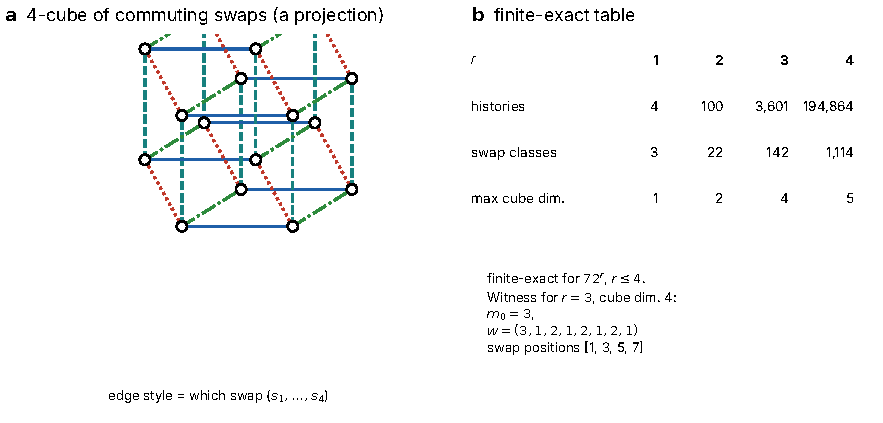
\includegraphics[width=\textwidth]{fig14_commuting_swaps}
\caption{\textbf{Commuting swaps and cubical faces (finite-exact data; the cube is drawn in projection).} (a) A projection of the $4$-cube formed by the sixteen histories obtained from the witness of \cref{prop:cubedim} by performing any subset of its four commuting exchanges; the four edge styles are the four exchanges $s_1,\dots,s_4$. It is a combinatorial $4$-cell and is not embedded in a Euclidean space of dimension $4$ by the drawing. (b) The table of \cref{tab:72r}.}\label{fig:cubes}
\end{figure}
\noindent The figure above is \cref{fig:cubes}; its caption states the exactness of what is drawn.
For $r=3$ the source-and-content groups number $141$ and the swap classes $142$: exactly one group of histories (source $15$, content $\{2,4,5,5,15\}$, endpoint $72^3$, two classes of four histories each) splits into two classes; for $r\le2$ classes and groups coincide. Over all non-squarefree endpoints $t\in[4,6000]$ with $H(t)\le4000$ (2\,354 endpoints), the endpoints at which some group of histories splits are exactly $1944,2400,4050,4320,5400$ (the first two sources of the pattern: source $2$, content $\{1,2,3,8\}$, endpoint $1944$, two classes of sizes $4$ and $1$; and the family of \cref{ex:src14}, endpoint $5400$). \stat{finite-exact}.
\prov{CW-0343}{D-T6}{FINITE-EXACT}{FINITE}
\begin{remark}[cube dimension is not homological degree]\label{rem:cubedeg}
The cube of \cref{thm:cube} is contractible, and a $d$-cube of commuting swaps contributes no homology of degree $d$ by its presence. For $r=3$ the complex $Q$ has cubes of dimension up to $4$ (four of them) but $\mathbb F_2$-Betti numbers $(142,368,3,0,0)$: homology lives in degrees $0,1,2$ only. The combinatorial cube dimension is an upper bound on the dimension of a cell, not an indication of any homological degree.
\end{remark}
\begin{proposition}[finite-exact: the groups are not always the classes]\label{prop:splitgroup}
The histories $(15;5,4,5,2,15)$ and $(15;15,2,4,5,5)$ have the same source, content $\{2,4,5,5,15\}$ and endpoint $72^3$ and lie in different swap classes; likewise $(2;1,2,3,8)$ and $(2;1,8,3,2)$ (endpoint $1944$).
\end{proposition}

\subsection{Dimension of an obstruction}
Let $C$ be a set of distinct labels and $m$ a source. Three numbers are attached to $(C,m)$: $d_{\mathrm{span}}=\rank_{\mathbb Q}\{\Delta(N):N\in C\}$ (the rank of the displacement vectors over \emph{all} primes); $d_{\mathrm{con}}=$ the number of primes $p$ such that relaxing the constraint at $p$ (replacing $v_p(m)$ by $\infty$, i.e.\ dropping $p$ from the thresholds) changes $\mathcal A(m)$; and $d_{\mathrm{top}}=$ the least size of a set $S$ of primes such that keeping only the constraints at $S$ preserves the Betti vector of $K_m$.
\begin{theorem}[passive coordinates]\label{thm:passive}
A prime that divides no label of $C$ never constrains: $\Delta_p(N)=2v_p(N+1)\ge0$ for $N\in C$, so $b_p(w)=0$ for every word $w$ over $C$. Hence admissibility, and every complex built from it, depends only on the active primes $\{p:p\mid N\text{ for some }N\in C\}$.
\end{theorem}
\begin{proof}
Immediate from \cref{thm:threshold}: $S_j(p)\ge0$ for all $j$.
\end{proof}
\prov{CW-0383}{B-T1}{PROVED}{FULL}
\begin{proposition}[the three dimensions differ]\label{prop:dims}
For $\{2,3,8,9\}$ at $72$: $(d_{\mathrm{span}},d_{\mathrm{con}},d_{\mathrm{top}})=(3,2,2)$; for $\{2,3,8,9,14\}$ at $1008$: $(4,2,2)$. In the first case the displacement vectors live in the primes $2,3,5$ (since $9+1=10$) and the active primes are $2,3$; in the second the displacement span has rank $4$ in the primes $2,3,5,7$, the active primes are $2,3,7$, the prime $7$ never constrains at $1008$ ($v_7(1008)=1$ and only the label $14$ consumes it), and the obstruction (the void of \cref{ex:void}) is already carried by the constraints at $\{2,3\}$.
\end{proposition}
\begin{proof}
Explicit exact computation: the ranks of the $\Delta$-matrices are $3$ and $4$; relaxing $2$ or $3$ changes $\mathcal A(m)$ and relaxing $7$ does not; keeping only the constraints at $\{2,3\}$ reproduces the Betti vectors $(1,1,0)$ and $(1,0,1,0)$, and no single prime does. See \cref{app:examples}.
\end{proof}
\prov{CW-0384}{B-T2}{PROVED}{FULL}
A rank-$4$ valuation realisation therefore carries a void whose obstruction is $2$-dimensional in the sense of constraints: the rank of the valuation span is not an obstruction dimension.
\begin{proposition}[irreducible multi-prime obstructions]\label{prop:irred}
Each of the following four statements about the route complex $K_m$ is an exact finite fact (replayed in \texttt{checks/}, with the admissible sets listed in \cref{app:examples}). For the content $C$ and source $m$ below, $K_m$ has the stated feature; and relaxing the constraint at any \emph{single} active prime makes $K_m$ contractible (Betti vector $(1,0,\dots,0)$), so every active prime is essential and the obstruction is genuinely $3$- (resp.\ $4$-)dimensional.
\begin{center}\small
\begin{tabular}{@{}llll@{}}\toprule
feature & content $C$ & source $m$ & active primes (all essential)\\\midrule
2 components & $\{2,3,4,5,6\}$ & $4$ & $2,3,5$\\
2 components & $\{2,3,4,5,6,7\}$ & $4$ & $2,3,5,7$\\
loop $(\beta_1=1)$ & $\{2,3,4,5,8\}$ & $32$ & $2,3,5$\\
loop $(\beta_1=1)$ & $\{2,3,4,5,6,7\}$ & $24$ & $2,3,5,7$\\\bottomrule
\end{tabular}
\end{center}
\end{proposition}
\prov{CW-0385}{B-T3}{PROVED}{FULL}
\emph{Irreducible means: relaxing any one active prime removes the obstruction.} In these examples the obstruction is a conjunction of independent single-prime blockers (every single relaxation trivialises it; none is a synergy of several primes). The number of active primes is not the dimension of the homology: the loop obstructions have first Betti number $1$ whatever their prime count, and the void has degree $2$ with constraint dimension $2$.
\begin{figure}[tbp]\centering
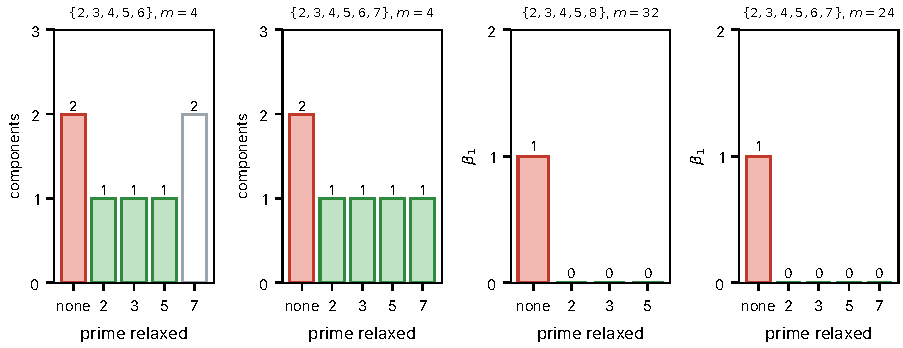
\includegraphics[width=\textwidth]{fig15_irreducible_obstructions}
\caption{\textbf{Irreducible prime-resource obstructions (exact).} For each of the four instances of \cref{prop:irred}: the number of components (panels 1--2) or the first Betti number (panels 3--4) of $K_m$ when nothing is relaxed (red bar) and when exactly one prime is relaxed (green bars). In panel~1 relaxing the passive prime $7$ (which does not constrain, by \cref{thm:passive}) is also shown and leaves $2$ components. Every active prime, relaxed alone, removes the obstruction. Theorem illustrated: \cref{prop:irred}, \cref{thm:passive}.}\label{fig:irreducible}
\end{figure}
\noindent The figure above is \cref{fig:irreducible}; its caption states the exactness of what is drawn.
\begin{proposition}[census of obstruction support; finite-exact, cited]\label{prop:supportcensus}
In the programme's census of route complexes with $k\le5$ labels (cap of $500$ resource vectors per content), disconnections occur with support $2,3,4$; loops with support $2,3$ (never $4$ for $k\le5$); voids only with support $2$; and the cut order (the least number of simultaneously relaxed primes that makes the complex contractible) is $1$ in about $17\,900$ non-trivial feature instances. This was not re-run here. Whether synergistic obstructions of cut order $\ge2$ exist is open.
\end{proposition}
\prov{CW-0386}{B-T4}{FINITE-EXACT}{FINITE}
\begin{problem}[open: repeated labels]\label{prob:repeated}
The complexes of this section and of \cref{sec:feasible} are defined for sets of distinct labels. For repeated labels the face structure of the arrangement graph needs a construction by chains of sub-multisets; none is given here, and \cref{thm:dual,thm:lower,thm:sphere} are not claimed for repeated labels. (The prefix-set form, the threshold law and \cref{thm:F2} do hold for repeated labels.)
\end{problem}

\section{Different-content endpoint relations}\label{sec:endpoints}
Up to now the content of a history, the multiset of its labels, was fixed. Here two histories with \emph{different} contents are compared. They can meet at one endpoint only through an arithmetic relation among the multipliers $R(N)$, and this relation is a lattice kernel.

\subsection{The valuation matrix and its kernel}
Fix a finite alphabet $A$ of labels. Let $\mathcal P$ be the set of primes dividing some $N$ or $N+1$ with $N\in A$, and let $V_A=(\Delta_p(N))_{p\in\mathcal P,\,N\in A}$ be the integer matrix of displacement vectors. For a history $h$ over $A$ let $c(h)\in\N^A$ be its content vector.
\begin{theorem}[endpoint equality is a kernel condition]\label{thm:kernel}
Two histories over $A$ from the same source have the same endpoint if and only if $V_A(c-c')=0$.
\end{theorem}
\begin{proof}
The endpoint is $m\prod_N R(N)^{c_N}$. A positive rational is determined by its $p$-adic valuations, $v_p(R(N))=\Delta_p(N)$, and a prime outside $\mathcal P$ has valuation $0$ for every $R(N)$, $N\in A$. Hence the endpoints agree iff $\sum_N(c_N-c'_N)\Delta_p(N)=0$ for all $p\in\mathcal P$.
\end{proof}
\prov{CW-0369}{D4-T1}{PROVED}{FULL}
\emph{Finite check.} Over all words of length $\le6$ from four sources, and on a box of $8\,110\,682$ content pairs of the programme's records, there is no violation (cited; the statement is a theorem, the check only guards the implementation). The content vectors of equal-endpoint histories form a coset of $\ker_{\Z}V_A$ intersected with $\N^A$ (a \emph{toric fibre}).

\begin{theorem}[every kernel vector is realised]\label{thm:realise}
Let $0\ne z\in\ker_{\Z}V_A$, $z=z^+-z^-$ with $z^\pm\ge0$, and let $m=\prod_N N^{|z_N|}$. Then every arrangement of the content $z^+$ and every arrangement of the content $z^-$ is admissible from $m$, and all of these histories have one endpoint, namely $m\prod_N R(N)^{z^+_N}=m\prod_N R(N)^{z^-_N}$. For arrangements $u$ of $z^+$ and $v$ of $z^-$ the pair is simultaneously admissible from a source $m'$ iff $\lcm(K(u),K(v))\mid m'$; the minimal sources of the relation form the antichain of the minimal $\lcm(K(u),K(v))$.
\end{theorem}
\begin{proof}
The content $z^+$ has $P(z^+)=\prod N^{z^+_N}$ dividing $m$, and likewise $P(z^-)$; by \cref{prop:sat} all arrangements are admissible. The endpoints coincide by \cref{thm:kernel}. The simultaneous admissibility criterion is \cref{thm:threshold} applied to $u$ and $v$.
\end{proof}
\prov{CW-0370}{D4-T2}{PROVED}{FULL}
The realising source is sufficient, not minimal. For the kernel vector $z$ below the pair $(2,2,3,3,3,3)$ against $(1^7)$ needs only the source $4$, whereas $\prod N^{|z_N|}=1\cdot2^2\cdot3^4=324$.

\begin{theorem}[the labels $\{1,2,3\}$]\label{thm:123}
$\ker_{\Z}V_{\{1,2,3\}}=\Z\,(7,-2,-4)$; equivalently $R(1)^7=R(2)^2R(3)^4=4^7=16384$.
\end{theorem}
\begin{proof}
Only the primes $2,3$ occur: $R(1)=4$, $R(2)=9/2$, $R(3)=16/3$ give
\[V=\begin{pmatrix}2&-1&4\\0&2&-1\end{pmatrix}\quad(\text{rows }p=2,3;\ \text{columns }N=1,2,3).\]
The rows are independent, so the kernel has rank $1$. From the second row $c_3=2c_2$ and from the first $2c_1-c_2+8c_2=0$, i.e.\ $c_1=-\tfrac72c_2$; the primitive generator is $(7,-2,-4)$. Direct evaluation: $(9/2)^2(16/3)^4=\frac{81}{4}\cdot\frac{65536}{81}=16384=4^7$.
\end{proof}
\prov{CW-0372}{D4-T4}{PROVED}{FULL}
\begin{example}[the benchmark merger from $4$]\label{ex:merger}
From the source $4$ the history $1^7$ passes through $4,16,64,256,1024,4096,16384,65536$. The content $\{2,2,3,3,3,3\}$ has exactly three admissible arrangements from $4$, namely $(2,2,3,3,3,3)$ through $4,18,81,432,2304,12288,65536$, and the arrangements $(2,3,2,3,3,3)$, $(2,3,3,2,3,3)$ (states shown in \cref{fig:merger}). All end at $4^8=65536$. Here $K(1^7)=1$, $K(2,2,3,3,3,3)=4$ and the smallest threshold of the three arrangements is $2$. \stat{finite-exact} in the arrangement count.
\end{example}
\begin{figure}[tbp]\centering
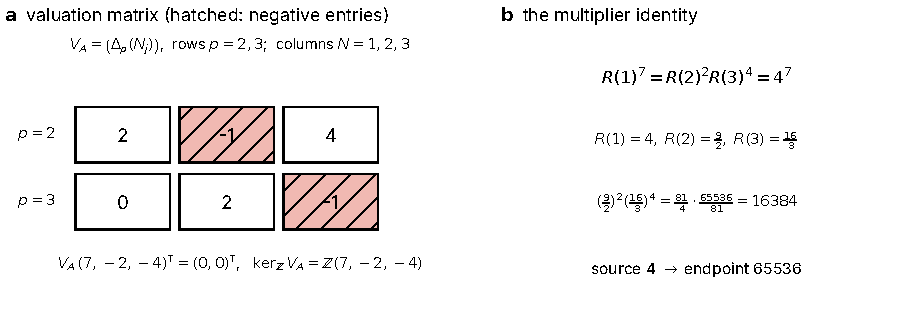
\includegraphics[width=\linewidth]{fig16_valuation_kernel}
\caption{\textbf{The valuation matrix of $\{1,2,3\}$ and the multiplier identity (exact).} (a) The matrix $V_A=(\Delta_p(N))$ with rows $p=2,3$ and columns $N=1,2,3$; entries are exact integers, negative entries are shaded and hatched. $V_A(7,-2,-4)^{\mathsf T}=0$ and the kernel over $\Z$ is $\Z(7,-2,-4)$. (b) The identity $R(1)^7=R(2)^2R(3)^4=4^7$ behind it; source $4$, endpoint $65536$. Theorem illustrated: \cref{thm:123}.}\label{fig:kernel}
\end{figure}
\noindent The figure above is \cref{fig:kernel}; its caption states the exactness of what is drawn.
\begin{figure}[tbp]\centering
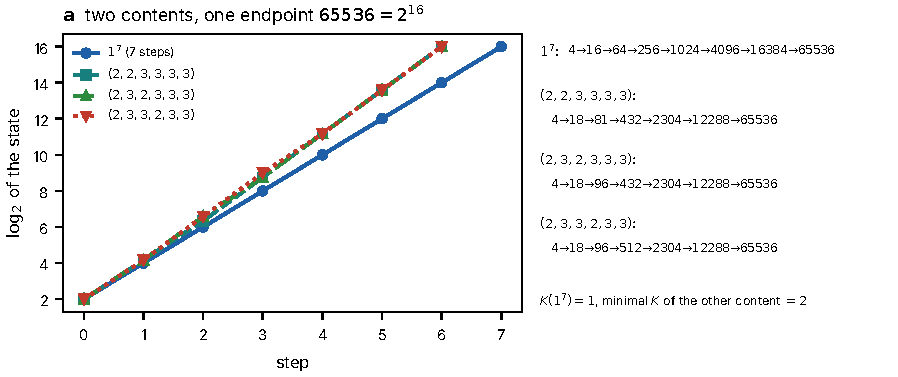
\includegraphics[width=\linewidth]{fig17_two_contents_65536}
\caption{\textbf{Two contents with one endpoint (exact, source $4$, endpoint $65536=2^{16}$).} (a) $\log_2$ of the state against the step for the history $1^7$ (circles, $7$ steps) and the three admissible arrangements of $\{2^2,3^4\}$ (squares, triangles; $6$ steps; dashed, dash-dotted and dotted lines respectively). The curves are different but meet at the endpoint. (b) The exact state sequences. $K(1^7)=1$; the smallest threshold among the three arrangements is $2$. Theorem illustrated: \cref{thm:realise}, \cref{thm:123}.}\label{fig:merger}
\end{figure}

\subsection{Geometry of the recombination: traces, area and closure}
Write $d_N=\Delta(N)\in\Z^{\mathcal P}$ and let the \emph{trace} of a history be the set of its visited states.
\begin{theorem}[trace and area]\label{thm:trace}
\begin{enumerate}[label=(\alph*)]
\item \emph{Trace injectivity.} Distinct histories from one source have distinct traces: the states strictly increase ($R(N)>1$), so ordering the trace recovers the state sequence, and consecutive ratios recover the labels because $R$ is injective.
\item \emph{Area potential.} For a word $w=(N_1,\dots,N_l)$ put $\Omega(w)=\sum_{i<j}d_{N_i}\wedge d_{N_j}$ (a bivector). An adjacent exchange of $N_k=a$ and $N_{k+1}=b$ changes $\Omega$ by exactly $-2\,d_a\wedge d_b$ (sharpening the factor $1$ recorded in the source); a block replacement $u\to v$ with $\sum d_u=\sum d_v$ changes $\Omega$ by $\Omega(v)-\Omega(u)$, independently of the prefix and the suffix. For arrangements of $\{2^2,3^4\}$ with $\mathrm{inv}$ the number of pairs with a $3$ before a $2$,
\[\Omega=\det(d_2,d_3)\,(8-2\,\mathrm{inv})\ (\text{in the }(v_2,v_3)\text{-plane}),\quad\det(d_2,d_3)=-7.\]
\item \emph{Closure triangle.} From the source $4$ the two histories $1^7$ and $(2,2,3^4)$, in the $(v_2,v_3)$-plane, bound the triangle with vertices $(2,0),(0,4),(16,0)$ (sides $2d_2$, $4d_3$ and $7d_1$) of area $28=4\,|\det(d_2,d_3)|$; the two paths meet only at their endpoints.
\end{enumerate}
\end{theorem}
\begin{proof}
(a) was argued above. (b) For an exchange, the terms $d_{N_i}\wedge d_{N_k}+d_{N_i}\wedge d_{N_{k+1}}$ with $i<k$ and $d_{N_k}\wedge d_{N_j}+d_{N_{k+1}}\wedge d_{N_j}$ with $j>k+1$ are symmetric in the exchanged pair, and the single pair term $d_a\wedge d_b$ becomes $d_b\wedge d_a=-d_a\wedge d_b$, which changes $\Omega$ by $-2d_a\wedge d_b$. For a block replacement, the cross terms between a prefix or suffix and the block are of the form $d_{N}\wedge\sum d_u$, and $\sum d_u=\sum d_v$. For $2^2 3^4$: pairs of equal labels contribute $0$; a pair $2$ before $3$ contributes $d_2\wedge d_3=-7$ and a pair $3$ before $2$ contributes $+7$, so $\Omega=-7(8-\mathrm{inv})+7\,\mathrm{inv}$. (c) The trace of $1^7$ is $(2,0),(4,0),\dots,(16,0)$; that of $(2,2,3,3,3,3)$ is $(2,0),(1,2),(0,4),(4,3),(8,2),(12,1),(16,0)$ (exact, verified from the state values). The triangle's area is $\frac12\cdot14\cdot4=28$; the second path stays in $v_3>0$ except at its endpoints.
\end{proof}
\prov{CW-0387}{B-T5}{PROVED}{FULL}
\begin{remark}[what $\Omega$ is and is not]
$\Omega$ is a function on vertices of the swap-and-rewrite graph, so the signed area of every closed combinatorial loop in that graph is $0$ by construction; it measures the \emph{area between two histories}, a weighted inversion statistic, not a homology class. It realises the $1$-skeleton and the bigons of the extended complex; higher cells are not realised as solids, and no coherence cells are present.
\end{remark}
\begin{proposition}[swap diamonds are nondegenerate; finite-exact]\label{prop:nondeg}
No two distinct labels $N<M\le400$ have parallel displacement vectors $d_N\parallel d_M$, so every swap diamond has nonzero area in some coordinate plane. The statement for all $N$ is open. \stat{finite-exact} (recomputed here: $0$ parallel pairs among labels $1,\dots,400$).
\end{proposition}
\prov{CW-0388}{B-T6}{FINITE-EXACT}{FINITE}

\subsection{The cube family}
Let $\mathrm{A}=1^7$ and $\mathrm B=2^2 3^4$ be the two sides of the relation of \cref{thm:123}. Starting at $4$, take $r$ successive blocks, each independently $\mathrm A$ or $\mathrm B$.
\begin{theorem}[block cube family]\label{thm:cubefam}
The $2^r$ histories so obtained all end at $4^{7r+1}$, have the $r+1$ contents $\mathrm A^{r-j}\mathrm B^j$ ($0\le j\le r$), and the cubical complex on the $2^r$ histories whose cells are the sets of independent block exchanges has $C(r,d)2^{r-d}$ cells of dimension $d$ and is contractible (the $r$-cube).
\end{theorem}
\begin{proof}
Each block multiplies by $4^7$ (via $\mathrm A$) or $R(2)^2R(3)^4=4^7$ (via $\mathrm B$) by \cref{thm:123}; the endpoint is $4\cdot4^{7r}$. A choice of blocks is a word in $\{\mathrm A,\mathrm B\}^r$; the cell count is that of the $r$-cube, which is contractible. The state before every block is a power of $4$, hence a multiple of $K(2,2,3,3,3,3)=4$, so the block $\mathrm B$ is admissible there by \cref{thm:threshold}; the block $\mathrm A=1^7$ is admissible from every state.
\end{proof}
\prov{CW-0373}{D4-T5}{PROVED}{FULL}
(The cell counts coincide with those of the cube; the homology is classical. The programme's verifier records Betti vectors $(1,0,\dots,0)$ for $r\le4$ \stat{finite-exact}.)

\subsection{Endpoint information and the kernel of content ambiguity}
For a fixed source $m$ and alphabet $A$, a history of content $c$ ends at $t$ with $v(t)-v(m)=V_Ac$, where $v$ denotes the vector of valuations at the primes $\mathcal P$ (\cref{thm:kernel}). The endpoint therefore determines the \emph{image} $V_Ac$, and two content vectors give the same endpoint exactly when they differ by an element of $\ker_{\Z}V_A$: the kernel coset is the content ambiguity of the endpoint. The rank of $V_A$ is a property of the alphabet and not of an individual endpoint. For the alphabet $\{1,2,3,8\}$ the matrix $V$ has rank $2$ and its kernel has rank $2$. The \emph{Graver candidates} found in the box of side $8$ are
\[\begin{gathered}z_1=(1,-4,0,2),\ z_2=(7,-2,-4,0),\ z_3=(3,1,-2,-1),\\ z_4=(4,-3,-2,1),\ z_5=(2,5,-2,-3)\end{gathered}\]
\stat{finite-exact} as a Graver list; the box is not a proof of completeness of the Graver basis (\cref{prop:graver}). What the endpoint does not determine, among contents, is the position within the kernel coset; block rewrites are the moves through that coset (\cref{sec:rewrites}).

\section{Block rewrites, source exposure and resource constraints}\label{sec:rewrites}
\subsection{The rewrite grammar and its threshold}
\begin{definition}[rewrite]\label{def:rewrite}
Let $z\in\ker_{\Z}V_A$ with $z=z^+-z^-$, and let $u$ and $v$ be arrangements of the contents $z^+$ and $z^-$. A \emph{block rewrite} is the replacement $p\cdot u\cdot s\to p\cdot v\cdot s$ of a contiguous block, where $p,s$ are words. Because $R(u)=R(v)$ the state after $p\cdot u$ equals the state after $p\cdot v$, so the suffix $s$ and the endpoint are unchanged. The \emph{rewrite graph} of a source $m$, an endpoint and a move set $M$ of kernel vectors has the admissible histories as vertices and the legal swaps and the legal block rewrites with $z\in\pm M$ as edges; its components are the \emph{rewrite classes}. A rewrite class is a union of swap classes.
\end{definition}
\begin{theorem}[block threshold]\label{thm:block}
Let $p\cdot u\cdot s$ be admissible from $m$. Then $p\cdot v\cdot s$ is admissible from $m$ iff $v$ is admissible from the state $x_p$ reached after $p$, i.e.\ iff $\lcm(K(p u s),K(p v s))\mid m$. The rewrite is thus an event local to the prefix state $x_p$: its executability depends on $x_p$ only through the valuations the block needs.
\end{theorem}
\begin{proof}
The prefix $p$ is common and admissible. After $p\cdot v$ the state is the same as after $p\cdot u$, so the suffix $s$ is admissible from it; the only remaining condition is the admissibility of $v$ from $x_p$. The equivalence with the $\lcm$ is the threshold law applied to the two words.
\end{proof}
\prov{CW-0371}{D4-T3}{PROVED}{FULL}
\emph{Check.} $425$ random cases of the criterion were replayed in this work, with $0$ violations (cited: $11\,000$ randomized tests in the programme's records).

\subsection{Saturation and the quotient description}
\begin{theorem}[saturation]\label{thm:saturation}
Suppose that the contents of the histories from $m$ to a fixed endpoint are connected by moves of a set $M$ (a Graver basis suffices) staying inside the fibre, and that $P(c)\mid m$ for every content $c$. Then the histories form a single rewrite class.
\end{theorem}
\begin{proof}
By \cref{prop:sat} every arrangement of every content is admissible, so each content is one swap class. For a move $z$ taking $c$ to $c'=c+z$, take any history of $c$, swap it into the form $u\cdot r$ with $u$ an arrangement of $z^-$ and $r$ the rest; then $v\cdot r$ is admissible by the same proposition and joins the two swap classes. Connectivity of the fibre under $M$ now gives connectivity of the rewrite graph. (A Graver basis is a Markov basis, \cite{Sturmfels1996,DiaconisSturmfels1998}.)
\end{proof}
\prov{CW-0374}{D4-T6a}{PROVED}{FULL}
\begin{proposition}[quotient description]\label{prop:quotient}
The rewrite classes are exactly the connected components of the graph whose nodes are the swap classes and whose edges are the \emph{exposed redexes}: a redex $u$ or $v$ occurring as a contiguous block in some word of a class whose replacement is admissible.
\end{proposition}
\begin{proof}
By \cref{def:rewrite}: a rewrite edge between two histories is by definition an exposed redex, and the classes of the graph with swap edges and rewrite edges are the components of the quotient by swap classes.
\end{proof}
\prov{CW-0375}{D4-T6b}{PROVED}{FULL}
\begin{corollary}[three obstruction types]\label{cor:trichotomy}
Below the saturation condition a rewrite graph can be disconnected for three separately observable reasons: (a) \emph{algebraic}, the content fibre is disconnected under $M$; (b) \emph{exposure}, contents are linked by a move of $M$ but no history has a contiguous redex because the context labels cannot be moved out of the block; (c) \emph{emptiness}, some content has no admissible history from $m$.
\end{corollary}
Algebraic obstructions hold at every source and are the subject of \cref{prop:graver}; exposure and emptiness are source-dependent and are separated for a test family below.

\subsection{Positive and negative completeness}
\begin{proposition}[three labels; finite-exact]\label{prop:T6c}
For the alphabet $\{1,2,3\}$, swaps together with the single move $1^7\leftrightarrow2^23^4$ connect all histories of equal source and endpoint, in the box $v_2(m)\le1$, $v_3(m)\le4$, $c_3\le8$ with fibre length $\ge2$ ($30$ fibres, $840$ fibre-source pairs, no disconnected pair; $16$ fibres and $364$ pairs re-checked independently in the programme). General $m$ is open: the fibres are the rank-one chains $c+t(7,-2,-4)$, so a proof would need an exposed redex for every consecutive pair of contents. \stat{finite-exact}.
\end{proposition}
\prov{CW-0376}{D4-T6c}{FINITE-EXACT}{FINITE}
\begin{proposition}[the Graver basis cannot be omitted]\label{prop:graver}
On the alphabet $\{1,2,3,8\}$ let $z_1=(1,-4,0,2)$ and $z_2=(7,-2,-4,0)$. The fibre $\{3^28,\ 1^32\}$ at endpoint $288=R(3)^2R(8)=R(1)^3R(2)$ contains two contents that are \emph{not} joined by $\pm z_1,\pm z_2$ and swaps: neither content admits a move (the contents $(0,0,2,1)$ and $(3,1,0,0)$ have $c_2\le1$, $c_3\le2$, $c_1\le3$, so none of $c\pm z_1$, $c\pm z_2$ is nonnegative). They are joined by the Graver vector $z_3=(3,1,-2,-1)=\bigl((3,1,0,0)-(0,0,2,1)\bigr)$. \stat{proved} for the explicit pair; the programme's census finds $498$ of $816$ fibres deficient for $\{z_1,z_2\}$ \stat{finite-exact}, not re-run here.
\end{proposition}
\prov{CW-0379}{D4-T7c}{PROVED}{FULL}
So generating the kernel is not enough: the move set must contain a Graver (Markov) basis for the fibre to be algebraically connected.

\subsection{An exposure dichotomy for all \texorpdfstring{$j$}{j}}
For $j\ge1$ consider the family $U_j=\{2^4,3^j\}$, $V_j=\{1,8^2,3^j\}$ with the move $2222\leftrightarrow$ any arrangement of $\{1,8,8\}$ (the kernel vector $z_1$); $R(2)^4=R(1)R(8)^2=3^8/2^4$. Write $a=v_2(m)$, $b=v_3(m)$.
\begin{theorem}[exposure dichotomy]\label{thm:Fj}
For every $j\ge1$: both contents have admissible histories from $m$ iff $b+8\ge j$ and $(a,b)\ne(0,0)$. In that case the swap-and-rewrite space is connected iff $b\ge1$ or $a\ge4$ (i.e.\ iff $3\mid m$ or $16\mid m$), and otherwise it has exactly two components, one swap class per content.
\end{theorem}
\begin{proof}
\emph{Realisability.} Each $2$ adds $2$ to $v_3$, each $8$ adds $4$, and each $3$ removes $1$, so the final $v_3$ is $b+8-j\ge0$. If $a=b=0$, then $U_j$ cannot start ($2$ needs $v_2\ge1$ and $3$ needs $v_3\ge1$) and $V_j$ stalls after the leading $1$ ($8$ needs $v_2\ge3$, $3$ needs $v_3\ge1$; a leading $1$ gives $v_2=2$ only). Otherwise explicit words exist: for $b\ge1$, $3,2,2,2,2,3^{j-1}$ and $3,1,8,8,3^{j-1}$; for $b=0,a\ge1$ (so $j\le8$), $2,3,2,2,2,3^{j-1}$ and $1,8,3,8,3^{j-1}$.

\emph{One swap class per content.} Let $A,B$ be coprime labels such that $2v_p(A+1)\ge v_p(B)$ for $p\mid B$ and $2v_q(B+1)\ge v_q(A)$ for $q\mid A$ (here $(2,3)$ and $(8,3)$: $2v_3(3)=2\ge1$, $2v_2(4)=4\ge1$, $2v_3(9)=4\ge1$). Claim: from any state, all admissible orderings of a multiset $\{A^s,B^t\}$ lie in one swap class. Induct on the length. Take admissible $A\cdot r$ and $B\cdot r'$. In $A\cdot r$ the first $B$ occurs after some $A$'s; it can be moved to the front of $r$ by legal adjacent swaps: at the state after the first $A$ we have $v_p\ge 2v_p(A+1)\ge v_p(B)$ for $p\mid B$, so $B$ is legal there; the $A$'s it passes only gain resources, since $\Delta_q(B)=2v_q(B+1)\ge0$ for $q\mid A$ and $q\nmid B$. Thus $A\cdot r$ is in the class of $A\cdot B\cdot r''$. Symmetrically $B\cdot r'$ is in the class of $B\cdot A\cdot r'''$. Both orders $AB$ and $BA$ are legal from the start state (each letter is legal at the start by assumption, and the other raises the resources of the first), with the same state afterwards; by induction the arrangements after them lie in one class, so the two classes coincide. For $V_j$ the label $1$ can be moved to the front by legal swaps (it divides everything and only raises $v_2$), so the claim applies after it.

\emph{Connectivity.} If $b\ge1$, both $3\cdot2222\cdot3^{j-1}$ and $3\cdot(1,8,8)\cdot3^{j-1}$ are admissible: after the leading $3$ the valuation $v_2\ge4$, the blocks leave $v_3=b+7\ge j-1$, and for $(1,8,8)$ the walk of $v_2$ is $\ge6,\ge3,\ge0$. They have one endpoint, so the block rewrite joins the two swap classes. If $a\ge4$, $b=0$ (so $j\le8$), then $2222\cdot3^j$ and $1\cdot8\cdot8\cdot3^j$ are admissible and the same argument applies.

\emph{Obstruction ($3\nmid m$, $a\le3$, $(a,b)\ne(0,0)$).} A label $3$ is applicable only after $v_3$ has been raised by a $2$ or an $8$. In $U_j$ all $2$s lie in the redex $2222$, in $V_j$ all $8$s lie in the redex (an arrangement of $\{1,8,8\}$). So no $3$ precedes a redex, the redex starts at position $0$ with $v_2=a\le3$, and: $2222$ needs $v_2\ge4$; the arrangements $(1,8,8)$, $(8,1,8)$ need $a\ge4$, $(8,8,1)$ needs $a\ge6$. No redex is ever exposed, so the two swap classes are not joined.
\end{proof}
\prov{CW-0391}{B-T9}{PROVED}{FULL}
\begin{figure}[tbp]\centering
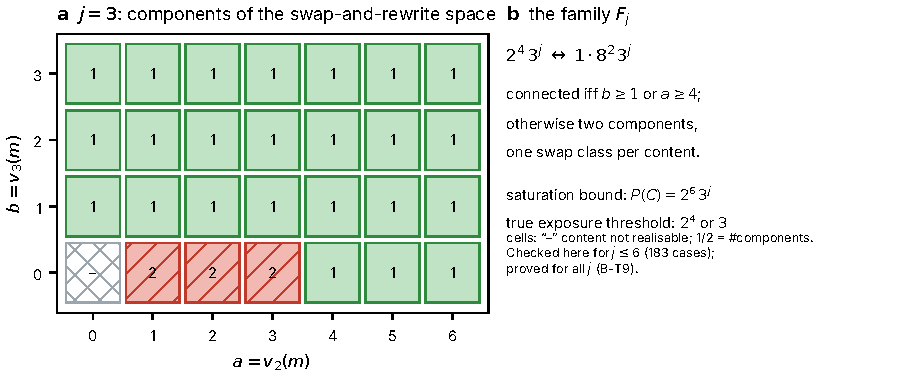
\includegraphics[width=0.78\linewidth]{fig18_rewrite_exposure}
\caption{\textbf{Components of the swap-and-rewrite space of $2^43^j\leftrightarrow1\cdot8^23^j$ for $j=3$ (finite-exact table, matching \cref{thm:Fj}).} The entry at $(a,b)=(v_2(m),v_3(m))$ is the number of components: $0$ (nothing realisable) at $(0,0)$, $2$ at $b=0$ and $a\in\{1,2,3\}$ (exposure obstruction), $1$ elsewhere. Colour is redundant with the printed integers. Theorem illustrated: \cref{thm:Fj}.}\label{fig:exposure}
\end{figure}
\noindent The figure above is \cref{fig:exposure}; its caption states the exactness of what is drawn.
\begin{remark}[supersession and sharpness]\label{rem:supersede}
The source release D4-T7b stated the dichotomy for $j\le8$ (finite-exact) and marked general $j$ open; the addendum proves it for all $j$ (the sufficient direction above, and the realisability bound $j\le b+8$, are what made the finite range natural). The saturation bound of \cref{thm:saturation} for this family is $2^63^j$ ($P(U_j)=2^43^j$, $P(V_j)=2^63^j$) while the true connectivity boundary is $3\mid m$ or $16\mid m$: the product bound is not sharp, and the sharp boundary is an exposure condition, not an all-arrangements condition.
\end{remark}
\prov{CW-0377}{D4-T7a}{PROVED}{FULL}
\prov{CW-0378}{D4-T7b}{MIXED}{SPLIT}
We recomputed the dichotomy for $j\le6$ over all $(a,b)$ with $a\le6$, $b\le j$ in this work, and it agrees ($183$ rows, no violation).

\subsection{Content-changing rewrites can create loops}
\begin{example}[the join example; exact]\label{ex:join}
$R(2)R(8)R(63)=R(5)R(9)R(35)=20736/7$. At the sources $m=280$ and $m=840$ the four histories $(2,63,8)$, $(8,63,2)$, $(5,9,35)$, $(35,9,5)$ have pairwise different traces; there is no legal swap, so the swap space is $4$ points with $4$ swap classes. The block replacements $(2,63,8)\leftrightarrow(5,9,35)$, $(2,63,8)\leftrightarrow(35,9,5)$, $(8,63,2)\leftrightarrow(5,9,35)$, $(8,63,2)\leftrightarrow(35,9,5)$ are all admissible and form a $4$-cycle: one rewrite class, cells $\{0:4,1:4\}$, $\mathbb F_2$-Betti vector $(1,1)$. A content-changing relation creates a loop out of a disconnected swap space.
\end{example}
\prov{CW-0380}{D4-T8a}{PROVED}{FULL}
\begin{problem}[open: homotopy type of extended complexes]\label{prob:extended}
The extended complex of histories with swaps and block rewrites has no coherence cells: braid hexagons and relations between overlapping moves are not filled, so its Betti numbers are invariants of this specific complex only. Its homotopy type, the effect of adding coherence cells, and Künneth-type behaviour for products of loop sides are open. A cycle in a restricted complex need not be a cycle in the complete one. \stat{open}.
\end{problem}
\prov{CW-0381}{D4-T8b}{OPEN}{OPEN}

\section{Occurrence-event invariants and prime-sensitive obstructions}\label{sec:events}
\subsection{The occurrence fibre}
For an integer state $x$ let $D(x)=\{d\ge2:\ d^2\mid x\}$ be its \emph{occurrence fibre}. A history $h=(x_0,x_1,\dots,x_l)$ induces the \emph{fibre sequence} $D(x_0),\dots,D(x_l)$, and for each index $d\ge2$ the incidence sequence $\rho_d(h)=([d\in D(x_i)])_{i}\in\{0,1\}^{l+1}$.
\begin{lemma}[orthant form]\label{lem:orthant}
$d\in D(x)$ iff $v_p(x)\ge2v_p(d)$ for every prime $p\mid d$. Hence $D(x)=D(x')$ iff $\lfloor v_p(x)/2\rfloor=\lfloor v_p(x')/2\rfloor$ for all $p$, and $\rho_d$ is the indicator of the valuation walk lying in the shifted orthant $O_d=\{v:v_p\ge2v_p(d)\ \forall p\mid d\}$; for a prime power $p^k$ it is the half-space $v_p\ge2k$.
\end{lemma}
\prov{CW-0356}{OCCURRENCE\_BRIDGE:Orthant-form}{PROVED}{FULL}
\begin{lemma}[labels are visible]\label{lem:L}
If $A\ne B$ are both admissible at $x$ then $D(T_Ax)\ne D(T_Bx)$. More precisely some prime $p$ has $|v_p(T_Ax)-v_p(T_Bx)|\ge2$, so $p^k$ lies in exactly one of the two fibres for suitable $k$.
\end{lemma}
\begin{proof}
Since $A+1\ne B+1$ some prime $p$ has, say, $v_p(A+1)>v_p(B+1)\ge0$. Then $p\nmid A$ and $\Delta_p(A)=2v_p(A+1)\ge2$. If $v_p(B+1)\ge1$ then $\Delta_p(B)=2v_p(B+1)$ and the difference is $\ge2$. If $v_p(B+1)=0$ then $\Delta_p(B)=-v_p(B)\le0$ and the difference is $\ge2v_p(A+1)\ge2$. A difference $\ge2$ in $v_p$ gives different integer parts of $v_p/2$.
\end{proof}
\begin{theorem}[faithfulness, locality, event locality]\label{thm:faith}
(a) For a fixed source the fibre sequence $F(h)$ determines the history $h$. (b) A legal swap changes exactly one entry of $F(h)$; hence the occurrence signature is never a swap invariant, and swaps preserve exactly the source, content, endpoint and all but one fibre. (c) If $d$ is lost at a step with label $N$ then $\gcd(d,N)>1$; if $d$ is born then $\gcd(d,N+1)>1$; the label $1$ never causes a loss.
\end{theorem}
\begin{proof}
(a) Induction on length: given $x_{j-1}$, \cref{lem:L} says the fibre $D(x_j)$ determines $N_j$ among the labels admissible at $x_{j-1}$. (b) A swap at position $i$ changes only the intermediate state; the two intermediate states are $T_Ax$ and $T_Bx$ with different fibres by \cref{lem:L}. (c) If $d\in D(x)\setminus D(Tx)$ there is $p\mid d$ with $v_p$ falling below $2v_p(d)$, so $\Delta_p(N)<0$, i.e.\ $p\mid N$. If $d$ is born then $\Delta_p(N)>0$ for some $p\mid d$, so $p\mid N+1$. Finally $\Delta_p(1)=2v_p(2)\ge0$.
\end{proof}
\prov{CW-0341}{D-T4}{PROVED}{FULL}
\emph{Corollary.} Histories with the same source and endpoint have pairwise different fibre sequences even when they are swap-equivalent: the endpoint keeps only the last entry. In the benchmark of $72$, $\rho_2(h_1)=(0,1,1,1)$ and $\rho_2(h_2)=(0,1,0,1)$ for the two swap-equivalent histories. Finite-exact check: $0$ collisions among $104$ histories and among $13\,950$ label pairs.
\begin{proposition}[local discrepancy]\label{prop:discrepancy}
For a legal swap with intermediate states $a=T_Ax$, $b=T_Bx$ and half-valuation vectors $e_p=\lfloor v_p/2\rfloor$, the changed entry differs by
\[|D(a)\,\triangle\,D(b)|=\prod_p(e_p(a)+1)+\prod_p(e_p(b)+1)-2\prod_p(\min(e_p(a),e_p(b))+1)>0,\]
because $D(a)\cap D(b)=D(\min(e(a),e(b)))$ and $|D(x)|=\prod_p(e_p(x)+1)-1$. The swap preserves $\rho_d$ iff $d\notin D(a)\triangle D(b)$, i.e.\ iff $a$ and $b$ lie on the same side of the orthant $O_d$.
\end{proposition}
\prov{CW-0357}{OCCURRENCE\_BRIDGE:Local-discrepancy}{PROVED}{FULL}

\subsection{Persistence-restricted swap connectivity}
For an index $d\ge2$ keep a legal swap in the \emph{preserve} mode iff $d\notin D(a)\triangle D(b)$; in the \emph{after-birth} mode iff that holds or $d$ occurs in none of $D(x_0),\dots,D(x_i)$. Both modes delete edges, so
\[\#\text{classes(unrestricted)}\le\#\text{classes(after birth)}\le\#\text{classes(preserve)}\]
(proved: deleting edges cannot decrease the component count; the after-birth edge set contains the preserve edge set). Restricting by all indices at once leaves no edge (\cref{lem:L}); a single index $d$ is the reduced, informative property.
\begin{table}[tbp]\centering\small
\begin{tabular}{@{}rrrrrrrrrr@{}}\toprule
$r$ & hist. & classes & pres.\ 2 & pres.\ 3 & pres.\ 4 & pres.\ 8 & aft.\ 2 & aft.\ 3 & pres.\ 12 / 36\\\midrule
1 & 4 & 3 & 4 & 4 & 4 & 3 & 4 & 3 & 3 / 3\\
2 & 100 & 22 & 36 & 51 & 62 & 54 & 32 & 24 & 43 / 33\\
3 & 3\,601 & 142 & 413 & 551 & 864 & 1\,009 & 355 & 239 & 678 / 493\\\bottomrule
\end{tabular}
\caption{\textbf{Swap classes of the complete histories of $72^r$ under persistence restriction (finite-exact; recomputed in this work).} ``pres.\ $d$'' and ``aft.\ $d$'' are the numbers of classes in the preserve and after-birth modes for the index $d$. The unrestricted counts are $3,22,142$.}\label{tab:persist}
\end{table}
\begin{proposition}[finite-exact: persistence restriction is strictly finer and not monotone in $d$]\label{prop:persist}
(1) Restricted connectivity is strictly finer than unrestricted already at $r=1$: for $d=2$ the histories $h_1,h_2$ of $72$ (swap-equivalent) are separated, $4$ classes instead of $3$. (2) The number of classes is not monotone along divisibility of $d$: for $r=3$ the index $d=12$ gives $678$ classes and $d=36$ gives $493$, though $12\mid36$ (for $r=2$: $43$ and $33$). (3) After-birth is coarser than preserve. \stat{finite-exact} for $r\le3$; no counting law in $r$ is known.
\end{proposition}
\prov{CW-0358}{OCCURRENCE\_BRIDGE:Results}{FINITE-EXACT}{FINITE}

\subsection{Churn}
For a history of length $l$ put $V_d=\sum_i|\rho_d(i+1)-\rho_d(i)|$ and $\chi_d=\tfrac12\bigl(V_d-|\rho_d(l)-\rho_d(0)|\bigr)$, the \emph{reduced churn} (the number of lost-and-regained or gained-and-lost excursions).
\begin{theorem}[churn bounds]\label{thm:churn}
(i) $\chi_d\le\lfloor l/2\rfloor$. (ii) A swap changes one entry of $\rho_d$, so $|\chi_d(h)-\chi_d(h')|\le1$ for swap-adjacent $h,h'$. (iii) If $\Delta_p(N)\ge0$ for all labels $N$ of $h$ and primes $p\mid d$, then $\rho_d$ is nondecreasing and $\chi_d=0$ (for instance $h_{\mathrm A}=1^7$). (iv) \emph{Dip lemma:} if $v_p$ dips to at least $2$ below its start value $a$ and ends at or above $a$, then $\chi_{p^{\lfloor a/2\rfloor}}\ge1$.
\end{theorem}
\begin{proof}
(i) $V_d\le l$ and $V_d\equiv|\rho_d(l)-\rho_d(0)|\pmod 2$, so $2\chi_d\le l$. (ii) Changing one interior entry of a $0/1$ sequence changes $V_d$ by at most $2$ and leaves the end values alone. (iii) $v_p$ is then nondecreasing for $p\mid d$, so $\rho_d$ is. (iv) With $k=\lfloor a/2\rfloor$: the start has $v_p=a\ge 2k$, so $\rho=1$; at the dip $v_p\le a-2<2k$ (as $2k\ge a-1$), so $\rho=0$; the end has $v_p\ge a\ge 2k$, so $\rho=1$; hence $V\ge2$ and $\chi\ge1$.
\end{proof}
\prov{CW-0389}{B-T7}{PROVED}{FULL}
\begin{theorem}[necessary churn of the merger]\label{thm:churnmerger}
For every source $m$ and every admissible arrangement of $\{2^2,3^4\}$ some $d$ has $\chi_d\ge1$, whereas $\chi_d(1^7)=0$ for all $d$. Hence every endpoint-preserving rewrite between $1^7$ and an arrangement of $\{2^2,3^4\}$ creates an occurrence gap.
\end{theorem}
\begin{proof}
The walk $v_3$ starts at $b=v_3(m)$ and has steps $+2$ (twice, labels $2$) and $-1$ (four times, labels $3$), ending at $b$, and stays $\ge0$. Take $d=3^k$, so $\rho_d=[v_3\ge2k]$.
\emph{Case 1:} the walk reaches $b+2$. Put $k=\lfloor b/2\rfloor+1\ge1$; then $2k\ge b+1>b$ and $2k\le b+2$, so $\rho=0$ at the start and the end, and $\rho=1$ at the moment of reaching $b+2$: $\chi\ge1$.
\emph{Case 2:} the walk stays $\le b+1$. Its first step cannot be $+2$, so it is $-1$ and the walk reaches $b-1$ (so $b\ge1$). If $b$ is even put $k=b/2\ge1$: $\rho=1$ at start and end ($v_3=b=2k$) and $\rho=0$ at $b-1$. If $b$ is odd and the walk reaches $b-2$ or lower put $k=(b-1)/2$: start and end have $\rho=1$ ($b\ge2k$), the low point has $v_3\le b-2<2k$. If $b$ is odd and the walk never goes below $b-1$, it can leave $b-1$ only by a $+2$ step, so it visits $b+1$; with $k=(b+1)/2$, $\rho=0$ at the start and end and $\rho=1$ at $b+1$. In each case $V_d\ge2$ and $\chi_d\ge1$. For $1^7$ every $\Delta_p(1)\ge0$, so \cref{thm:churn}(iii) gives $\chi_d=0$.
\end{proof}
\prov{CW-0390}{B-T8}{PROVED}{FULL}
\emph{Check.} All arrangements for $v_2(m)\le8$, $v_3(m)\le6$ ($690$ admissible cases) and the monotone and dip statements ($1126$ and $2162$ cases) were replayed with no violation. In the block cube family from $4$ the total churn at source $4$ equals the number of $\mathrm B$-blocks; the minimum number of churning indices over all sources and arrangements within the tested index set is $5$ (cited).

\subsection{Information across rewrites}
\begin{proposition}[births minus losses is a rewrite invariant]\label{prop:births}
Let $\mathrm{births}$ and $\mathrm{losses}$ be the numbers of index-birth and index-loss events along a history. Then $\mathrm{births}-\mathrm{losses}=|D(x_l)|-|D(x_0)|$ depends only on the endpoint and the source, so it is a rewrite invariant. The fibre sequences are \emph{not} rewrite invariants (rewrites change lengths). In the cube family of \cref{thm:cubefam}, $\mathrm A$ has $(\mathrm{births},\mathrm{losses})=(7,0)$ and $\mathrm B$ has $(14,7)$, with difference $7$ each; the $2^r$ histories of the cube family are pairwise distinguished by their fibre sequences for $r\le4$, while the pairs $(\mathrm{births},\mathrm{losses})$ take $2,4,8,15,24$ distinct values for $r=1,\dots,5$, so that the pair is a faithful label only for $r\le3$. The first statement is proved by telescoping; the numerical statements are \stat{finite-exact} and cited.
\end{proposition}
\prov{CW-0382}{D4-T9}{PROVED}{FULL}
The endpoint fixes the image $V_Ac$ and leaves the position in the kernel coset free; block rewrites move within that coset, and a telescoping invariant such as $\mathrm{births}-\mathrm{losses}$ depends on the endpoint alone and so cannot see that position.

\subsection{A separator of swap classes by one occurrence index}
\begin{theorem}[the order of $2$ and $4$; proved-scoped]\label{thm:R3T3}
Let $A$ be a set of distinct labels with $A\cap\{1,2,4\}=\emptyset$, let the source be $4$ and the content $C=\{2,4\}\cup A$. For an admissible arrangement $w$ of $C$ put $I(w)=1$ if $2$ precedes $4$ and $I(w)=0$ otherwise. Then $I$ is constant on swap classes. Consequently the number of swap classes is at least the number of values of $I$ that occur.
\end{theorem}
\begin{proof}
A swap exchanging two labels other than the pair $\{2,4\}$ does not change the relative order of $2$ and $4$. A legal swap of $2$ and $4$ requires them to be adjacent with $8=2\cdot4$ dividing the state $x$ before the pair (\cref{prop:diamond}). If the pair is not at the first two positions, the first label of the history lies in $A$; but at the source $4$ the only applicable labels are the divisors $1,2,4$ of $4$, and $A$ contains none of them. So the pair occupies the first two positions and $x=4$, and $8\nmid4$.
\end{proof}
\provx{R3-T3}{CW-0413/0414 (proposed co-located proof)}{proved-scoped}{full}
\begin{example}[the family from endpoint $9000$]\label{ex:R3T3}
For $A=\{5,9\}$ the content $\{2,4,5,9\}$ ends at $9000$ and has $2$ swap classes, each of $2$ histories: $\{(2,9,4,5),(2,9,5,4)\}$ with $I=1$ and $\{(4,5,2,9),(4,5,9,2)\}$ with $I=0$ (\cref{fig:occur}). For $A=\{3,5,9\}$ (endpoint $48000$) there are $3$ classes (sizes $1,3,4$) with $I$-values $1,1,0$, and for $A=\{3,5,6,9\}$ (endpoint $392000$) there are $3$ classes (sizes $5,8,14$) with the same $I$-values: $I$ separates the pair of values but is not a complete invariant. In a sweep over all $39$ subsets $A\subseteq\{3,\dots,12\}$ of size $1$ to $3$ the invariance of $I$ holds in all cases ($0$ violations); the number of classes is $1$ for $24$ contents, $2$ for $14$ and $3$ for $1$, and both values of $I$ occur for $14$. \stat{finite-exact}. The classification of the classes beyond $I$ is not given.
\end{example}
\begin{figure}[tbp]\centering
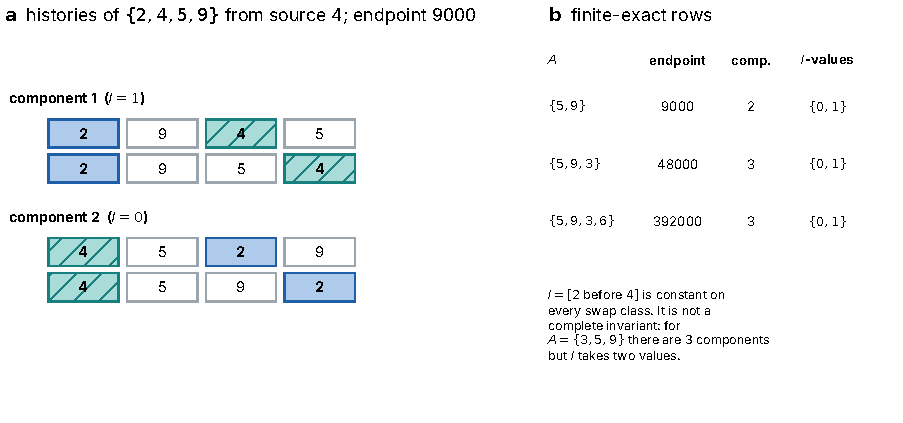
\includegraphics[width=\linewidth]{fig19_occurrence_events}
\caption{\textbf{The order of $2$ and $4$ separates swap classes (finite-exact data, theorem exact).} (a) The four histories of the content $\{2,4,5,9\}$ from source $4$ (endpoint $9000$) grouped into the two swap classes; the labels $2$ (light fill) and $4$ (hatched) are marked, with $I=[2$ before $4]$. (b) The three rows computed: the sets $A$, endpoints, number of components and values of $I$; for $A=\{3,5,9\}$ there are $3$ components but $I$ takes two values only. Theorem illustrated: \cref{thm:R3T3}.}\label{fig:occur}
\end{figure}
\begin{remark}[a corrected statement]\label{rem:B2T9}
The square-root content $\sigma(x)=\prod_pp^{\lfloor v_p(x)/2\rfloor}$ has $D(x)$ as its set of divisors $\ge2$, and along every SELECT-II edge $\sigma'/\sigma=(N+1)/c>1$ with $c\le N$ the product of the prime powers $p^{\lfloor\cdot/2\rfloor}$ or $p^{\lceil\cdot/2\rceil}$ taken from $N$ (the programme's B2-T9, ``no silent step''). The inclusion $D(x)\subsetneq D(x')$ that was once stated with it does \emph{not} hold, as the accepted erratum records: $4\to18$ has $D(4)=\{2\}$ and $D(18)=\{3\}$. The occurrence fibre is therefore not monotone along histories, which is why churn is a meaningful quantity. \stat{cited}.
\end{remark}

\section{Relation to individual-state geometry}\label{sec:geometry}
Manuscript~I~\cite{PaperI} attached to a single state a geometry; here only the integer part is needed. Two facts about it are taken from the programme's releases and are \stat{cited}, not re-proved.
\begin{itemize}[leftmargin=1.6em,itemsep=1pt]
\item \emph{Collapse of integer state geometry (B2-T1).} For an integer $x$ put $\sigma(x)=\prod_pp^{\lfloor v_p(x)/2\rfloor}$. The complete geometric record of $x$ is a function of $\sigma(x)$ alone, equivalent to the occurrence set $D(x)$ (the divisors $\ge2$ of $\sigma(x)$); all its topological invariants are trivial and the move complex $\Kmove(x)$ of an integer state is contractible. What varies between integers is dimension, shape, the $f$-vector and the inclusion order.
\item \emph{Different objects.} $\Kmove(x)$ lives on the occurrence set of one state; the history complexes of this manuscript live on admissible words from a fixed source. They are not identified.
\end{itemize}
\begin{proposition}[obstruction to detecting histories by state homology]\label{prop:A4T7}
Every integer endpoint $E$ of a SELECT-II history has $\Kmove(E)$ contractible (cited). Hence no homological invariant of $\Kmove(E)$ can detect the component structure of the histories ending at $E$. Witnesses: the endpoints $9000$, $48000$, $392000$ have $2$, $3$, $3$ components of histories with contents $\{2,4\}\cup A$, $A=\{5,9\},\{5,9,3\},\{5,9,3,6\}$ (source $4$; recomputed in this work, \cref{ex:R3T3}), and the order bit $I=[2\text{ before }4]$ is constant on components and takes both values (\cref{thm:R3T3}); each $\Kmove(E)$ has $\mathbb F_2$-Betti vector $(1,0,0,0)$ (cited). \stat{cited} for the contractibility; \stat{finite-exact} for the component counts.
\end{proposition}
\provx{A4-T7}{GEO\_HD\_BRIDGE\_v004:A4-T7 (obstruction)}{cited}{cited}
\begin{figure}[tbp]\centering
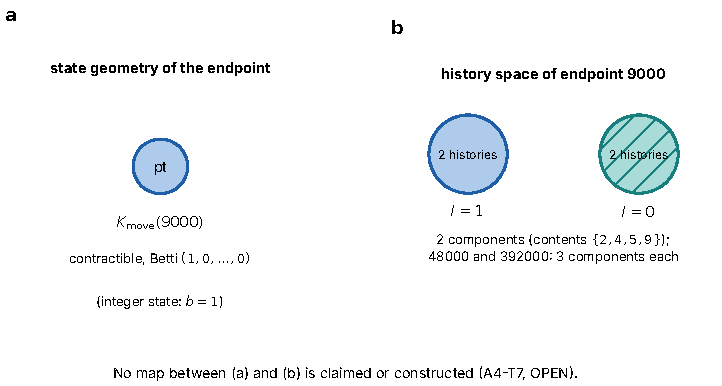
\includegraphics[width=\linewidth]{fig20_state_vs_history}
\caption{\textbf{Contractible state geometry against a disconnected history space (schematic, data finite-exact).} (a) The state geometry of the endpoint $9000$ is a point up to homotopy: $\Kmove(9000)$ is contractible with Betti vector $(1,0,0,0)$ (cited). (b) The swap-class structure of the histories of $\{2,4,5,9\}$ from source $4$ ending at $9000$: two components of two histories each, distinguished by $I$ (exact). The picture is schematic; no map between (a) and (b) is claimed or constructed. Theorem illustrated: \cref{prop:A4T7}.}\label{fig:state}
\end{figure}
\noindent The figure above is \cref{fig:state}; its caption states the exactness of what is drawn.
What is \emph{not} established. No functor, map or inequality between $H_*(\Kmove)$ and the homology of a history complex is claimed. A direct comparison would need an invariant of rational states that is meaningful for histories without extending SELECT-II, which the model boundary of this manuscript excludes; the question whether such an invariant exists is open (\cref{sec:synthesis}). The only integer-level connection proved here is the occurrence-event one: the fibre sequence of a history is built from $D(x_i)=D(\sigma(x_i))$ (\cref{thm:faith}), so the state geometry of the visited states determines the fibre sequence while the state geometry of the endpoint alone does not (\cref{prop:A4T7}).

\section{Synthesis, conclusions and open problems}\label{sec:synthesis}
\subsection{Mathematical conclusions}
\begin{enumerate}[leftmargin=2em,itemsep=2pt]
\item \emph{The endpoint forgets the history.} For the endpoint $72$ the four histories have three contents and three swap classes (\cref{fig:objects}). In general, for a fixed source and alphabet, the endpoint determines the image $V_Ac$, i.e.\ the content only modulo $\ker_{\Z}V_A$ (\cref{thm:kernel}), and says nothing about order.
\item \emph{Order is governed by one divisibility.} Admissibility of a word is $K(w)\mid m$ (\cref{thm:threshold}); every swap, class and component statement of \cref{sec:swaps,sec:feeding} is a statement about the induced subgraph of the arrangement graph on $\{w:K(w)\mid m\}$.
\item \emph{Same content, different classes.} Resource contention, not numerical incompatibility, separates arrangements: $(14,3,2)$ and $(2,3,14)$ commute numerically and are not connected by admissible swaps at $14$ (\cref{thm:2314}); this is the hexagon deadlock of \cref{thm:T3}.
\item \emph{Topology.} The permutohedral route complex has the homology of the nerve of the infeasible arrangements (\cref{thm:dual}); complementary infeasible pairs give the homology of $S^{k-3}$ (\cref{thm:sphere}), realised by a loop for $\{2,3,8,9\}$ at $72$ and a void for $\{2,3,8,9,14\}$ at $1008$. Cube dimension is not homological degree (\cref{rem:cubedeg}), and the dimension of an obstruction in terms of prime resources is not the rank of the valuation span (\cref{prop:dims}).
\item \emph{Rewrites.} Different-content histories with the same endpoint are the integer kernel of $V_A$, all kernel vectors are realised, a rewrite is local to a prefix state (\cref{thm:block}), and below the saturation threshold three obstruction types occur; the exposure threshold of the family $2^4 3^j\leftrightarrow1\cdot8^23^j$ is exactly $3\mid m$ or $16\mid m$ for every $j$ (\cref{thm:Fj}).
\item \emph{Occurrence events.} The fibre sequence determines the history (\cref{thm:faith}); the merger $1^7\leftrightarrow2^23^4$ necessarily creates occurrence gaps (\cref{thm:churnmerger}); the pair order of $2$ and $4$ separates swap classes at endpoints $9000,48000,392000$ although the state geometry of those endpoints is contractible (\cref{prop:A4T7}).
\end{enumerate}

\subsection{Corrections and sharpenings made in this manuscript}\label{sec:corrections}
\begin{itemize}[leftmargin=1.6em,itemsep=1pt]
\item The all-arrangements statement is an exact equivalence, $P(C)\mid m$ (\cref{prop:sat}); the converse for \emph{connectivity} is false ($\{2,3,14\}$ at $28$ is connected though $2\cdot3\cdot14=84\nmid28$).
\item The sphere statement is homological: complementary infeasible pairs give the homology of $S^{k-3}$, the homotopy type is not proved (\cref{thm:sphere}).
\item The area potential changes by $-2\,d_a\wedge d_b$ under an adjacent exchange, not $d_a\wedge d_b$ (\cref{thm:trace}); the $\{2^2,3^4\}$ formula $-7(8-2\,\mathrm{inv})$ is consistent only with the factor $2$.
\item The exposure dichotomy is proved for every $j$ (\cref{thm:Fj}); the source's finite range $j\le8$ is superseded.
\item B2-T9 originally stated an inclusion $D(m)\subsetneq D(m')$, which fails ($4\to18$); the correct statement is the strict increase of $\sigma$ (\cref{rem:B2T9}).
\item \emph{Status of the $\{2,3,N\}$ converse.} In the source release the arithmetic part of D-T9 is proved and the converse (a split source exists only if $N\equiv2,3\pmod6$) is finite-exact for $4\le N\le400$. In this manuscript the converse is proved for every $N\ge4$: \cref{thm:23N}(a) shows by the block factorisation \cref{thm:F2} that $\nu\le1$ unless the feeding digraph is strongly connected, i.e.\ unless $N\equiv2,3\pmod6$, and \cref{thm:23N}(b) classifies the split sources in the strongly connected case by \cref{thm:T3}. The source's finite range is retained as corroboration only.
\item Cited, not re-run: the census of $k\le5$ labels (cut order $1$ in about $17\,900$ instances), the loop converse for $4\le N<M\le60$, the $498$ of $816$ deficient fibres, the births-and-losses table.
\end{itemize}

\subsection{Open problems}
\begin{problem}[swap-class classification]\label{prob:classify}
Classify the swap classes of all contents, beyond the contents of one to three labels and the family $\{2,3,N\}$: the structure of the $\lcm$-closure $L(C)$ and the maximal number of components for $k$ labels. \stat{open} (D-Q1).
\end{problem}
\prov{CW-0513}{D-Q1}{OPEN}{OPEN}
\begin{problem}[common futures]\label{prob:futures}
Unbounded statements on common futures of histories (two histories with a common continuation) are known only as bounded regression data. \stat{open} (D-Q3).
\end{problem}
\prov{CW-0515}{D-Q3}{OPEN}{OPEN}
\begin{problem}[image of the fibre-sequence map]\label{prob:image}
Which sequences of fibres occur as fibre sequences of histories? \Cref{thm:faith} shows injectivity but not the image. \stat{open} (D-Q4).
\end{problem}
\prov{CW-0516}{D-Q4}{OPEN}{OPEN}
\begin{problem}[overlapping cells]\label{prob:overlap}
The Independence Lemma fills cubes for non-overlapping exchanges only (\cref{rem:hexagon}). A complex with cells for overlapping moves, the effect of coherence cells on the extended complex of \cref{prob:extended}, and $319$ triples with pairwise diamonds but no triple cell for $m<400$ (cited) are open. \stat{open} (D-Q5).
\end{problem}
\prov{CW-0517}{D-Q5}{OPEN}{OPEN}
\begin{problem}[interface to the next stage]\label{prob:interface}
An invariant of rational states meaningful for histories without extending SELECT-II (\cref{sec:geometry}); the relation of the history complexes to the programme's later stages. \stat{open} (D-Q6).
\end{problem}
\prov{CW-0518}{D-Q6}{OPEN}{OPEN}
Further problems stated in the text: growth of $H(72^r)$ and of the maximal cube dimension (\cref{prob:growth}); whether $K_m$ is always a wedge of spheres (\cref{prob:wedge}); complexes for repeated labels (\cref{prob:repeated}); homotopy type and Künneth behaviour of extended complexes (\cref{prob:extended}); synergistic obstructions of cut order $\ge2$ (\cref{prop:supportcensus}); a proof of connectivity for $\{1,2,3\}$ at all sources (\cref{prop:T6c}); parallel displacement vectors for all $N$ (\cref{prop:nondeg}).

\clearpage
\phantomsection\addcontentsline{toc}{section}{References}
\begin{thebibliography}{99}\small\raggedright
\bibitem{PaperI} UNNS Research Collective, \emph{Arithmetic Transport and Dimensional Obstructions in UNNS Occurrence Geometry}, Manuscript~I of the programme GEO-HD-1, version~0.2 (2~Nov.\ 2026); file \texttt{PAPER\_I\_TRANSPORT\_v0.2.pdf}, SHA-256 \texttt{5f7c0809db2006b419c7f7490c1aca01e984b5ad5f814ae3209e44728f312a68}.
\bibitem{FoundI} UNNS Substrate programme, \emph{Mathematical Foundations of the UNNS Substrate, Volume~I: Generative Arithmetic and Structural Reachability} (the grammar SELECT-II and the occurrence set). Source: \texttt{ukbbi/UNNS}, commit \texttt{9a021346b2b3d964523440d2737b9d0c4ddbb3e5}, \texttt{projects/UNNS\_MATH\_FOUNDATIONS/Manuscript}.
\bibitem{FoundII} UNNS Substrate programme, \emph{Mathematical Foundations of the UNNS Substrate, Volume~II: Collective Dynamics, Prime Rigidity, and Effective Predictability}. Same commit and path as~\cite{FoundI}. Cited only for the existence of the rational dynamics FIELD-I, which this manuscript does not use.
\bibitem{RefColl} Foundations reference collection v001 (SELECT-I/II, FIELD-I v001--v012; frozen), \texttt{ukbbi/UNNS}, commit \texttt{bb8b12d753c600c597feb00df17fe139c7cc65fa} (23 Oct.\ 2026), \texttt{projects/UNNS\_MATH\_FOUNDATIONS/sources}.
\bibitem{HD1} GEO-HD-1 research collection, snapshot \texttt{a88f31487f3b05c9db297dcd1192d56eea2b0c7d} (the pin named in the programme specification; not independently verified in this work). The release archives from which the records of this manuscript are taken, with their SHA-256 as computed on the files supplied for this work:
\begin{itemize}[leftmargin=1.4em,itemsep=1pt,topsep=2pt]\footnotesize
\item\texttt{GEO\_HD\_1D\_v001} \texttt{c532b7410f3bf9d437f9f172b3e56029cd9f7bab5b2ac0c0e533713155eaf7a4};
\item\texttt{GEO\_HD\_1D\_v002} \texttt{8baf463c07bb5285dd53b355aee05a0f841c068ba3ae4794f3702adff6a4bae0};
\item\texttt{GEO\_HD\_1D\_v003} \texttt{65dbb281e4c75d625b6cf3e4bcb8262d7d42e68d0c476fbba225fcde744a4706};
\item\texttt{GEO\_HD\_1D\_v004} \texttt{e0390e2a2f88eaeb11042de09fd056741ed98f94318de708d308faa090f05b5b};
\item\texttt{GEO\_HD\_BRIDGE\_v001} \texttt{e99472809928f4a23fb292f60759965159c7a4db5f018d56748ccac328719395};
\item\texttt{GEO\_HD\_BRIDGE\_v002} \texttt{012ead97e5b8854cd5218417d46f0e388d927b6d59d5f6e75a8cc343f5dd4955} (with the accepted erratum \texttt{GEO\_HD\_BRIDGE\_v002\_ERRATUM\_B2-T9.md});
\item\texttt{GEO\_HD\_BRIDGE\_v003} \texttt{6fba87af9f3096772e43f4ac77fa8d55aea9e242eeef241081a987b567d5d5a8};
\item\texttt{GEO\_HD\_BRIDGE\_v004} \texttt{cfb31157a39666d1a4bbb33b280ec626c7de2c141e8232da43c8b934b8affff4};
\item\texttt{GEO\_HD\_BRIDGE\_v005} \texttt{50e342821d7a5f760c5127df348e97f3a4d4d3bf34bf60e1019d6336f28c5d03}.
\end{itemize}
\bibitem{Mazurkiewicz1987} A.~Mazurkiewicz, Trace theory, in: W.~Brauer, W.~Reisig, G.~Rozenberg (eds.), \emph{Petri Nets: Applications and Relationships to Other Models of Concurrency}, Lecture Notes in Computer Science~255, Springer, 1987, 278--324.
\bibitem{DiekertRozenberg1995} V.~Diekert, G.~Rozenberg (eds.), \emph{The Book of Traces}, World Scientific, 1995.
\bibitem{CartierFoata1969} P.~Cartier, D.~Foata, \emph{Probl\`emes combinatoires de commutation et r\'earrangements}, Lecture Notes in Mathematics~85, Springer, 1969.
\bibitem{Newman1942} M.~H.~A. Newman, On theories with a combinatorial definition of ``equivalence'', \emph{Ann.\ of Math.} (2) \textbf{43} (1942), 223--243.
\bibitem{BaaderNipkow1998} F.~Baader, T.~Nipkow, \emph{Term Rewriting and All That}, Cambridge University Press, 1998.
\bibitem{Graver1975} J.~E. Graver, On the foundations of linear and integer linear programming~I, \emph{Math.\ Programming} \textbf{9} (1975), 207--226.
\bibitem{Sturmfels1996} B.~Sturmfels, \emph{Gr\"obner Bases and Convex Polytopes}, University Lecture Series~8, American Mathematical Society, 1996.
\bibitem{DiaconisSturmfels1998} P.~Diaconis, B.~Sturmfels, Algebraic algorithms for sampling from conditional distributions, \emph{Ann.\ Statist.} \textbf{26} (1998), 363--397.
\bibitem{Hatcher2002} A.~Hatcher, \emph{Algebraic Topology}, Cambridge University Press, 2002 (nerve theorem, Corollary~4G.3; Alexander duality, Proposition~3.46).
\bibitem{Ziegler1995} G.~M. Ziegler, \emph{Lectures on Polytopes}, Graduate Texts in Mathematics~152, Springer, 1995 (the permutohedron, Example~0.10).
\bibitem{Bjorner1995} A.~Bj\"orner, Topological methods, in: R.~L. Graham, M.~Gr\"otschel, L.~Lov\'asz (eds.), \emph{Handbook of Combinatorics}, vol.~2, Elsevier/MIT Press, 1995, 1819--1872.
\bibitem{Kozlov2008} D.~N. Kozlov, \emph{Combinatorial Algebraic Topology}, Algorithms and Computation in Mathematics~21, Springer, 2008.
\bibitem{Pratt1991} V.~Pratt, Modeling concurrency with geometry, in: \emph{Proc.\ 18th ACM Symp.\ on Principles of Programming Languages (POPL)}, 1991, 311--322.
\bibitem{FajstrupEtAl2016} L.~Fajstrup, E.~Goubault, E.~Haucourt, S.~Mimram, M.~Raussen, \emph{Directed Algebraic Topology and Concurrency}, Springer, 2016.
\end{thebibliography}
\paragraph{On the references.} UNNS sources are cited at the commits and archive hashes fixed by the programme; repository access during this work was read-only and the pinned repositories were not fetched from the environment in which the manuscript was prepared. The external literature is cited by author, title and publication data. It is cited only for \emph{resemblance} of structure (commutation classes, rewriting systems, Markov bases, directed topology) and for the standard theorems named; nothing in the manuscript is proved by appeal to an equivalence with those theories.

\appendix
\section{Source theorem crosswalk}\label{app:crosswalk}
\subsection{Provenance records}
Every result of this manuscript that restates a record of the programme's crosswalk carries a line ``\emph{Source record}'' in the text. The table below is generated at build time from these lines (\texttt{scripts/make\_appmap.py}); it lists the crosswalk row, the source identifier, the status recorded in the crosswalk, the proof treatment of the allocation (\textsc{full}: proof given here; \textsc{finite}: exact finite computation, presented as such; \textsc{open}: stated as a problem; \textsc{split}: proved part and finite-exact part stated separately), and the section and number at which it appears. Rows appearing twice are restated in two places.
\begin{center}\scriptsize
\begin{longtable}{@{}llllll@{}}\toprule
CW row & source id & status & treatment & section & number\\\midrule\endhead
\texttt{A4-T7} & \texttt{GEO\_HD\_BRIDGE\_v004:A4-T7 (obstruction)} & cited & cited & 12 & 12.1\\
\texttt{CW-0336} & \texttt{D-T0} & PROVED & FULL & 3 & 3.1\\
\texttt{CW-0337} & \texttt{D-W} & PROVED & FULL & 2 & 2.4\\
\texttt{CW-0338} & \texttt{D-T1} & PROVED & FULL & 4 & 4.5\\
\texttt{CW-0339} & \texttt{D-T2} & PROVED & FULL & 3 & 3.4\\
\texttt{CW-0340} & \texttt{D-T3} & PROVED & FULL & 8 & 8.1\\
\texttt{CW-0341} & \texttt{D-T4} & PROVED & FULL & 11 & 11.3\\
\texttt{CW-0342} & \texttt{D-T5} & PROVED & FULL & 5 & 5.9\\
\texttt{CW-0343} & \texttt{D-T6} & FINITE-EXACT & FINITE & 8 & 8.4\\
\texttt{CW-0344} & \texttt{D-T7} & PROVED & FULL & 4 & 4.2\\
\texttt{CW-0345} & \texttt{D-T7'} & PROVED & FULL & 5 & 5.2\\
\texttt{CW-0346} & \texttt{D-T8} & PROVED & FULL & 5 & 5.5\\
\texttt{CW-0347} & \texttt{D-T9} & MIXED & SPLIT & 6 & 6.10\\
\texttt{CW-0348} & \texttt{D-T10} & PROVED & FULL & 5 & 5.8\\
\texttt{CW-0349} & \texttt{THEOREMS\_V002:Census-FINITE-EXACT-results} & FINITE-EXACT & FINITE & 6 & 6.12\\
\texttt{CW-0350} & \texttt{NF} & PROVED & FULL & 6 & 6.2\\
\texttt{CW-0351} & \texttt{F2} & PROVED & FULL & 6 & 6.3\\
\texttt{CW-0351} & \texttt{F2} & PROVED & FULL & 6 & 6.4\\
\texttt{CW-0352} & \texttt{Hub-descent} & PROVED & FULL & 6 & 6.6\\
\texttt{CW-0353} & \texttt{CONNECTIVITY:Census-on-three-labels-FINITE} & FINITE-EXACT & FINITE & 6 & 6.6\\
\texttt{CW-0354} & \texttt{T3} & PROVED & FULL & 6 & 6.7\\
\texttt{CW-0355} & \texttt{OBSTRUCTIONS:Parameter-family-2-3-N-PROV} & PROVED & FULL & 6 & 6.10\\
\texttt{CW-0356} & \texttt{OCCURRENCE\_BRIDGE:Orthant-form} & PROVED & FULL & 11 & 11.1\\
\texttt{CW-0357} & \texttt{OCCURRENCE\_BRIDGE:Local-discrepancy} & PROVED & FULL & 11 & 11.4\\
\texttt{CW-0358} & \texttt{OCCURRENCE\_BRIDGE:Results} & FINITE-EXACT & FINITE & 11 & 11.5\\
\texttt{CW-0359} & \texttt{T-DUAL} & PROVED & FULL & 7 & 7.3\\
\texttt{CW-0360} & \texttt{T-LOWER} & PROVED & FULL & 7 & 7.4\\
\texttt{CW-0361} & \texttt{T-SPHERE} & PROVED & FULL & 7 & 7.5\\
\texttt{CW-0362} & \texttt{ROUTE\_TOPOLOGY:Cubical-versus-permutohedral} & FINITE-EXACT & FINITE & 7 & 7.10\\
\texttt{CW-0363} & \texttt{ROUTE\_TOPOLOGY:Census-FINITE-EXACT-contents} & FINITE-EXACT & FINITE & 7 & 7.12\\
\texttt{CW-0364} & \texttt{ROUTE\_TOPOLOGY:Statement-of-the-general-conje} & OPEN & OPEN & 7 & 7.13\\
\texttt{CW-0365} & \texttt{D6-T1} & PROVED & FULL & 4 & 4.2\\
\texttt{CW-0366} & \texttt{(P) Prefix-set form} & PROVED & FULL & 4 & 4.3\\
\texttt{CW-0367} & \texttt{(G) Dependence on the source} & PROVED & FULL & 4 & 4.4\\
\texttt{CW-0368} & \texttt{D6-T2} & PROVED & FULL & 4 & 4.7\\
\texttt{CW-0369} & \texttt{D4-T1} & PROVED & FULL & 9 & 9.1\\
\texttt{CW-0370} & \texttt{D4-T2} & PROVED & FULL & 9 & 9.2\\
\texttt{CW-0371} & \texttt{D4-T3} & PROVED & FULL & 10 & 10.2\\
\texttt{CW-0372} & \texttt{D4-T4} & PROVED & FULL & 9 & 9.3\\
\texttt{CW-0373} & \texttt{D4-T5} & PROVED & FULL & 9 & 9.8\\
\texttt{CW-0374} & \texttt{D4-T6a} & PROVED & FULL & 10 & 10.3\\
\texttt{CW-0375} & \texttt{D4-T6b} & PROVED & FULL & 10 & 10.4\\
\texttt{CW-0376} & \texttt{D4-T6c} & FINITE-EXACT & FINITE & 10 & 10.6\\
\texttt{CW-0377} & \texttt{D4-T7a} & PROVED & FULL & 10 & 10.9\\
\texttt{CW-0378} & \texttt{D4-T7b} & MIXED & SPLIT & 10 & 10.9\\
\texttt{CW-0379} & \texttt{D4-T7c} & PROVED & FULL & 10 & 10.7\\
\texttt{CW-0380} & \texttt{D4-T8a} & PROVED & FULL & 10 & 10.10\\
\texttt{CW-0381} & \texttt{D4-T8b} & OPEN & OPEN & 10 & 10.11\\
\texttt{CW-0382} & \texttt{D4-T9} & PROVED & FULL & 11 & 11.8\\
\texttt{CW-0383} & \texttt{B-T1} & PROVED & FULL & 8 & 8.7\\
\texttt{CW-0384} & \texttt{B-T2} & PROVED & FULL & 8 & 8.8\\
\texttt{CW-0385} & \texttt{B-T3} & PROVED & FULL & 8 & 8.9\\
\texttt{CW-0386} & \texttt{B-T4} & FINITE-EXACT & FINITE & 8 & 8.10\\
\texttt{CW-0387} & \texttt{B-T5} & PROVED & FULL & 9 & 9.5\\
\texttt{CW-0388} & \texttt{B-T6} & FINITE-EXACT & FINITE & 9 & 9.7\\
\texttt{CW-0389} & \texttt{B-T7} & PROVED & FULL & 11 & 11.6\\
\texttt{CW-0390} & \texttt{B-T8} & PROVED & FULL & 11 & 11.7\\
\texttt{CW-0391} & \texttt{B-T9} & PROVED & FULL & 10 & 10.8\\
\texttt{CW-0513} & \texttt{D-Q1} & OPEN & OPEN & 13 & 13.1\\
\texttt{CW-0514} & \texttt{D-Q2} & OPEN & OPEN & 3 & 3.6\\
\texttt{CW-0515} & \texttt{D-Q3} & OPEN & OPEN & 13 & 13.2\\
\texttt{CW-0516} & \texttt{D-Q4} & OPEN & OPEN & 13 & 13.3\\
\texttt{CW-0517} & \texttt{D-Q5} & OPEN & OPEN & 13 & 13.4\\
\texttt{CW-0518} & \texttt{D-Q6} & OPEN & OPEN & 13 & 13.5\\
\texttt{R3-T3} & \texttt{CW-0413/0414 (proposed co-located proof)} & proved-scoped & full & 11 & 11.9\\
\bottomrule\end{longtable}
\end{center}

\subsection{Allocation notes}
\begin{itemize}[leftmargin=1.6em,itemsep=2pt]
\item \emph{Accepted transfer.} The records B-T1 to B-T9 (\texttt{CW-0383} to \texttt{CW-0391}) are history and rewrite theory carried by the bridge releases; their transfer from the stage-III allocation to this manuscript is recorded in \texttt{crosswalk/PAPER\_II\_DERIVED\_ALLOCATION.md}.
\item \emph{Proposed co-location.} R3-T3 (\texttt{CW-0413}, \texttt{CW-0414}), the separator $I=[2\text{ before }4]$, is restated with a complete proof in \cref{thm:R3T3}; its allocation remains with the stage-III manuscript, and the proof here is a proposed co-located one (printed as ``derived allocation'').
\item \emph{Cited, not re-proved.} B2-T9 (as corrected by the accepted erratum) in \cref{rem:B2T9}; B2-T1 and A4-T7 in \cref{sec:geometry}. No identification of state geometry with history topology is claimed.
\item \emph{Mixed rows.} D-T9 ($\{2,3,N\}$: the arithmetic statement proved, the converse finite-exact in the source; here the converse is proved for all $N\ge4$ by the factorisation theorem and the three-label classification, \cref{thm:23N}, and the source's range $N\le400$ is retained as corroboration) and D4-T7b (superseded for all $j$ by B-T9, \cref{thm:Fj}).
\item \emph{Release pins.} Archives and commits are listed in the references~\cite{HD1,FoundI,RefColl}.
\end{itemize}

\section{Complete arithmetic examples}\label{app:examples}
All tables of this appendix are generated by \texttt{scripts/make\_appB\_data.py} with the independent exact engine \texttt{scripts/engine.py} and are reproduced verbatim from its output (exact integer arithmetic, no floating point). Section numbers in the headings below refer to this manuscript.
\subsection*{B.1 The four complete histories of 72}
\begin{center}\small\begin{tabular}{@{}rlll@{}}\toprule source & word & states & content\\\midrule
1 & $(1,1,2)$ & $1\to 4\to 16\to 72$ & $1, 1, 2$\\
1 & $(1,2,1)$ & $1\to 4\to 18\to 72$ & $1, 1, 2$\\
3 & $(3,2)$ & $3\to 16\to 72$ & $2, 3$\\
10 & $(5)$ & $10\to 72$ & $5$\\
\bottomrule\end{tabular}\end{center}
\subsection*{B.2 Thresholds of the arrangements of $\{2,3,14\}$}
\begin{center}\small\begin{tabular}{@{}lr@{}}\toprule arrangement $w$ & $K(w)$\\\midrule
$(2,3,14)$ & 14\\
$(2,14,3)$ & 28\\
$(3,2,14)$ & 21\\
$(3,14,2)$ & 21\\
$(14,2,3)$ & 28\\
$(14,3,2)$ & 14\\
\bottomrule\end{tabular}\end{center}
\subsection*{B.3 Complexes of Section 7 and Section 8}
\paragraph{$\{2,3,8,9\}$ at $72$ (loop)}Admissible arrangements: 16 of 24. Swap classes: 1. Betti vector of $K_m$ over $\mathbb F_2$: $(1,1,0)$; $f$-vector $(16,20,4)$.
\paragraph{$\{2,3,8,9,14\}$ at $1008$ (void)}Admissible arrangements: 96 of 120. Swap classes: 1. Betti vector of $K_m$ over $\mathbb F_2$: $(1,0,1,0)$; $f$-vector $(96,180,98,12)$.
\paragraph{$\{2,3,4,5,6\}$ at $4$ (\cref{prop:irred})}Admissible arrangements: 10 of 120. Swap classes: 2. Betti vector of $K_m$ over $\mathbb F_2$: $(2,0,0)$; $f$-vector $(10,9,1)$.
Component sizes: 4, 6.
\paragraph{$\{2,3,4,5,6,7\}$ at $4$ (\cref{prop:irred})}Admissible arrangements: 24 of 720. Swap classes: 2. Betti vector of $K_m$ over $\mathbb F_2$: $(2,0,0)$; $f$-vector $(24,29,7)$.
Component sizes: 12, 12.
\paragraph{$\{2,3,4,5,8\}$ at $32$ (\cref{prop:irred})}Admissible arrangements: 30 of 120. Swap classes: 1. Betti vector of $K_m$ over $\mathbb F_2$: $(1,1,0)$; $f$-vector $(30,41,11)$.
Component sizes: 30.
\paragraph{$\{2,3,4,5,6,7\}$ at $24$ (\cref{prop:irred})}Admissible arrangements: 87 of 720. Swap classes: 1. Betti vector of $K_m$ over $\mathbb F_2$: $(1,1,0,0)$; $f$-vector $(87,151,70,6)$.
Component sizes: 87.
\subsection*{B.4 The overlap hexagon}
The content $\{1,2,4\}$ from source $2$: admissible arrangements $(1,2,4)$, $(1,4,2)$, $(2,1,4)$ of 6; $P(C)=8\nmid 2$.

\subsection*{B.5 The dimensions of an obstruction (\cref{prop:dims})}
For $C=\{2,3,8,9\}$ at $72$ the displacement vectors over the primes $2,3,5$ are $\Delta(2)=(-1,2,0)$, $\Delta(3)=(4,-1,0)$, $\Delta(8)=(-3,4,0)$ and $\Delta(9)=(2,-2,2)$ (since $10=2\cdot5$); the rank is $3$. For $C=\{2,3,8,9,14\}$ at $1008=2^4\cdot3^2\cdot7$ the label $14$ adds $\Delta(14)=(-1,2,2,-1)$ in the primes $(2,3,5,7)$ ($15=3\cdot5$), and the rank over $2,3,5,7$ is $4$. The prime $7$ is consumed once, by the unique label $14$, and $v_7(1008)=1$, so it never constrains; relaxing $2$ or $3$ changes the admissible set and relaxing $7$ does not. Keeping only the constraints at $\{2,3\}$ reproduces the Betti vector $(1,0,1,0)$ of the full complex, and neither $\{2\}$ nor $\{3\}$ alone does.
\subsection*{B.6 The kernel merger and the cube family}
Source $4$: $1^7$ has states $4,16,\dots,65536$; $(2,2,3,3,3,3)$ has states $4,18,81,432,2304,12288,65536$; $(2,3,2,3,3,3)$ and $(2,3,3,2,3,3)$ reach the same endpoint (\cref{ex:merger}). The block cube family has $2^r$ histories ending at $4^{7r+1}$, e.g.\ $r=1,2,3$: $65536$, $1073741824$, $17592186044416$ ($=4^8,4^{15},4^{22}$), replayed in this work.

\section{History-complex construction}\label{app:complex}
\subsection*{C.1 The permutohedral route complex}
Let $C=\{N_1,\dots,N_k\}$ be distinct labels and $\mathcal A(m)\subseteq S_k$ the set of admissible arrangements. The boundary complex $\partial P_k$ of the permutohedron~\cite{Ziegler1995} has as faces the ordered set partitions $(B_1|\dots|B_s)$ of $\{1,\dots,k\}$, $s\ge2$; its vertices are the $k!$ arrangements (all blocks singletons) and a face contains an arrangement when the arrangement lists the blocks in order. The \emph{route complex} $K_m$ is the full subcomplex on $\mathcal A(m)$: a face is present iff every arrangement it contains is admissible. The cubical complex $Q_m$ instead has as cells the sets of pairwise non-overlapping legal swaps of one history (\cref{lem:indep}); the two coincide on the $1$-skeleton, differ in higher cells, and the hexagon of three labels is a $2$-cell of $K_m$ but not of $Q_m$.
\subsection*{C.2 Chain complexes and the check $\partial^2=0$}
Both complexes are used with $\mathbb F_2$ coefficients and cellular boundary $\partial\sigma=\sum_{\tau\subset\sigma,\ \dim\tau=\dim\sigma-1}\tau$. For the face poset of $\partial P_k$ (a regular CW sphere) and for the cubical complex every codimension-two incidence is a diamond, so $\partial^2=0$; in addition the program asserts $\partial_{i-1}\partial_i=0$ numerically before each rank computation (\texttt{scripts/topo.py}, function \texttt{betti\_from\_boundaries}), and the Betti numbers are checked against the Euler characteristic of the $f$-vector in every table of this manuscript. Those checks passed in every reported case (for instance $16-20+4=0$ and $1-1+0=0$ for the loop of $\{2,3,8,9\}$; $96-180+98-12=2$ and $1-0+1-0=2$ for the void).
\subsection*{C.3 Implementation}
Cells of $K_m$ are enumerated as ordered set partitions whose linear extensions all lie in $\mathcal A(m)$; ranks over $\mathbb F_2$ are computed by Gaussian elimination on bit-packed rows. For repeated labels no such construction is given (\cref{prob:repeated}). General background on complexes of this type: \cite{Bjorner1995,Kozlov2008}.

\section{Kernel and rewrite calculations}\label{app:kernel}
\subsection*{D.1 The valuation matrix of $\{1,2,3,8\}$}
Rows $p=2,3$, columns $N=1,2,3,8$:
\[V=\begin{pmatrix}2&-1&4&-3\\0&2&-1&4\end{pmatrix},\]
with kernel of rank $2$ over $\Z$. Each of the five Graver candidates of \cref{sec:endpoints} satisfies $Vz=0$:
\begin{center}\small\begin{tabular}{@{}lrr@{}}\toprule $z$ & $2$-row & $3$-row\\\midrule
$(1,-4,0,2)$ & $2+4+0-6$ & $0-8+0+8$\\
$(2,5,-2,-3)$ & $4-5-8+9$ & $10+2-12$\\
$(3,1,-2,-1)$ & $6-1-8+3$ & $2+2-4$\\
$(4,-3,-2,1)$ & $8+3-8-3$ & $-6+2+4$\\
$(7,-2,-4,0)$ & $14+2-16$ & $-4+4$\\\bottomrule\end{tabular}\end{center}
(each row sums to $0$).
\subsection*{D.2 The $\{3^28,\ 1^32\}$ pair}
$R(3)^2R(8)=\bigl(\tfrac{16}3\bigr)^2\tfrac{81}8=288=R(1)^3R(2)=64\cdot\tfrac92$. The difference of the content vectors is $(3,1,0,0)-(0,0,2,1)=(3,1,-2,-1)=z_3$.
\subsection*{D.3 The family $2^43^j\leftrightarrow1\cdot8^23^j$}
$R(2)^4=\tfrac{6561}{16}=\tfrac{3^8}{2^4}$ and $R(1)R(8)^2=4\cdot\tfrac{6561}{64}=\tfrac{3^8}{2^4}$. The valuation walks: a leading $3$ adds $4$ to $v_2$; $2$ changes $(v_2,v_3)$ by $(-1,+2)$; $8$ by $(-3,+4)$; $1$ by $(+2,0)$; $3$ by $(+4,-1)$. For $b\ge1$ the words $3,2,2,2,2,3^{j-1}$ and $3,1,8,8,3^{j-1}$ have $v_3$ trajectories $b-1,b+1,b+3,b+5,b+7,\dots$ and $b-1,b-1,b+3,b+7,\dots$, both ending at $b+8-j$.
\subsection*{D.4 The join example}
$R(2)R(8)R(63)=\tfrac92\cdot\tfrac{81}8\cdot\tfrac{4096}{63}=\tfrac{20736}7=\tfrac{36}5\cdot\tfrac{100}9\cdot\tfrac{1296}{35}=R(5)R(9)R(35)$. At $m=280$ the histories $(2,63,8)$, $(8,63,2)$, $(5,9,35)$, $(35,9,5)$ end at $280\cdot20736/7=829440$.

\section{Supplementary proofs}\label{app:proofs}
\subsection*{E.1 The threshold is the least admissible source}
\emph{Claim.} The admissible sources of a word $w$ are exactly the multiples of $K(w)$, and $K(w)$ is the least. \emph{Proof.} By \cref{thm:threshold}, $w$ is admissible from $m$ iff $K(w)\mid m$. \qed
\subsection*{E.2 Euler characteristic of $Q$ for $72^r$}
The $f$-vectors $(4,1)$, $(100,96,11)$, $(3601,6366,2832,294,4)$ give $\chi=4-1=3$, $100-96+11=15$ and $3601-6366+2832-294+4=-223$; the Betti vectors $(3)$, $(22,7)$, $(142,368,3)$ give $3$, $22-7=15$, $142-368+3=-223$. The agreement is a consistency check on the boundary matrices, not a proof of the Betti numbers (which are exact finite computations).
\subsection*{E.3 Two small proofs used in the text}
\emph{The pair $\{2,4\}$ cannot be exchanged except at the start.} By \cref{prop:diamond} the exchange of $a,b$ at a state $x$ is legal iff $ab\mid x$. For $\{2,4\}$ this requires $8\mid x$. At the source $4$ with every other label outside $\{1,2,4\}$ the pair must open the history (\cref{thm:R3T3}), $x=4$ and $8\nmid4$.

\emph{The invariance of $\mathrm{births}-\mathrm{losses}$.} Along a history $\mathrm{births}_i-\mathrm{losses}_i=|D(x_i)|-|D(x_{i-1})|$ at step $i$, because $D(x_i)\setminus D(x_{i-1})$ are the births and $D(x_{i-1})\setminus D(x_i)$ the losses; summing telescopes to $|D(x_l)|-|D(x_0)|$, which depends on the source and the endpoint only.

\end{document}
